\documentclass[10pt]{article}\usepackage[]{graphicx}\usepackage[]{color}
% maxwidth is the original width if it is less than linewidth
% otherwise use linewidth (to make sure the graphics do not exceed the margin)
\makeatletter
\def\maxwidth{ %
  \ifdim\Gin@nat@width>\linewidth
    \linewidth
  \else
    \Gin@nat@width
  \fi
}
\makeatother

\definecolor{fgcolor}{rgb}{0.345, 0.345, 0.345}
\newcommand{\hlnum}[1]{\textcolor[rgb]{0.686,0.059,0.569}{#1}}%
\newcommand{\hlstr}[1]{\textcolor[rgb]{0.192,0.494,0.8}{#1}}%
\newcommand{\hlcom}[1]{\textcolor[rgb]{0.678,0.584,0.686}{\textit{#1}}}%
\newcommand{\hlopt}[1]{\textcolor[rgb]{0,0,0}{#1}}%
\newcommand{\hlstd}[1]{\textcolor[rgb]{0.345,0.345,0.345}{#1}}%
\newcommand{\hlkwa}[1]{\textcolor[rgb]{0.161,0.373,0.58}{\textbf{#1}}}%
\newcommand{\hlkwb}[1]{\textcolor[rgb]{0.69,0.353,0.396}{#1}}%
\newcommand{\hlkwc}[1]{\textcolor[rgb]{0.333,0.667,0.333}{#1}}%
\newcommand{\hlkwd}[1]{\textcolor[rgb]{0.737,0.353,0.396}{\textbf{#1}}}%
\let\hlipl\hlkwb

\usepackage{framed}
\makeatletter
\newenvironment{kframe}{%
 \def\at@end@of@kframe{}%
 \ifinner\ifhmode%
  \def\at@end@of@kframe{\end{minipage}}%
  \begin{minipage}{\columnwidth}%
 \fi\fi%
 \def\FrameCommand##1{\hskip\@totalleftmargin \hskip-\fboxsep
 \colorbox{shadecolor}{##1}\hskip-\fboxsep
     % There is no \\@totalrightmargin, so:
     \hskip-\linewidth \hskip-\@totalleftmargin \hskip\columnwidth}%
 \MakeFramed {\advance\hsize-\width
   \@totalleftmargin\z@ \linewidth\hsize
   \@setminipage}}%
 {\par\unskip\endMakeFramed%
 \at@end@of@kframe}
\makeatother

\definecolor{shadecolor}{rgb}{.97, .97, .97}
\definecolor{messagecolor}{rgb}{0, 0, 0}
\definecolor{warningcolor}{rgb}{1, 0, 1}
\definecolor{errorcolor}{rgb}{1, 0, 0}
\newenvironment{knitrout}{}{} % an empty environment to be redefined in TeX

\usepackage{alltt}
\usepackage{graphicx, verbatim}
\usepackage[utf8]{inputenc}
\usepackage{amsmath}
\usepackage{amssymb}
\usepackage{amscd}
\usepackage{lipsum}
\usepackage{blindtext}
\usepackage{todonotes}
\usepackage[tableposition=top]{caption}
\usepackage{ifthen}
\usepackage{caption}
\setlength{\textwidth}{6.5in} 
\setlength{\textheight}{9in}
\setlength{\oddsidemargin}{0in} 
\setlength{\evensidemargin}{0in}
\setlength{\topmargin}{-1.5cm}
\setlength{\parindent}{0cm}
\usepackage{setspace}
\usepackage{float}
\usepackage{fancyhdr}
\usepackage{tabularx}
\usepackage{soul} 

\usepackage{hyperref}
\hypersetup{
  colorlinks   = true, %Colours links instead of ugly boxes
  urlcolor     = blue, %Colour for external hyperlinks
  linkcolor    = blue, %Colour of internal links
  citecolor   = red %Colour of citations
}

\usepackage[backend=biber ,sorting=none]{biblatex}
\bibliography{references}
\begin{filecontents*}{references.bib}
\end{filecontents*}


%\fancyhf{}
\rfoot{Group 2 \thepage}
\singlespacing
\usepackage[affil-it]{authblk} 
\usepackage{etoolbox}
\usepackage{lmodern}

% \makeatletter
% \renewcommand{\maketitle}{\bgroup\setlength{\parindent}{16pt}
% \begin{flushleft}
%   \textbf{\@title}
% 
%   \@author
% \end{flushleft}\egroup
% }

%\renewcommand\Authfont{\fontsize{14}{18.4}\selectfont}
%\makeatother

% \pagestyle{fancy}
% \rfoot{Page \thepage}
 %\thispagestyle{empty} 



\IfFileExists{upquote.sty}{\usepackage{upquote}}{}
\begin{document}


\title{\LARGE Professional Development and Research Skills - CMM507 Coursework  \\ Group 2: Plastic Pollution in Oceans}

\author{ALEXANDER RITCHIE, \textit{\href{1911218@rgu.ac.uk}{1911218@rgu.ac.uk}};\\ GEORGIOS ORFANAKIS, \textit{\href{1903446@rgu.ac.uk}{1903446@rgu.ac.uk}};\\ KAREN JEWELL, \textit{\href{1415410@rgu.ac.uk}{1415410@rgu.ac.uk}};\\ ROSHI SHRESTHA, \textit{\href{1903445@rgu.ac.uk}{1903445@rgu.ac.uk}};\\ STUART WATT, \textit{\href{1501869@rgu.ac.uk}{1501869@rgu.ac.uk}}}

\maketitle
% \begin{flushleft} \today \end{flushleft} 
\noindent\rule{16cm}{0.4pt}
%\underline{\hspace{3cm}
\ \\
%\thispagestyle{empty}

\section{Introduction}



\subsection{Problem Statement}\label{statement}

Plastic pollution is a serious problem in the marine environment where they have major impact on marine and human health. In order to understand the depth of the problem, it is essential to understand the amount and composition of marine litter. This can help in applying various mitigation strategies. This section will include:
\begin{itemize}
\item An overview of the marine pollution
\item Motivation behind this topic
\item Aim and objectives of this report
\end{itemize}


\subsection{Overview}\label{over}

Marine pollution is a major global issue which impacts on environment, economy and human health. Although marine pollution is caused by many different materials, plastics consist of 60-80\% of the marine litter. Synthetic organic polymer derived from polymerisation of monomers extracted from oil and gas make up the plastics.\cite{DERRAIK2002} \cite{RIOS2007} The lightweight feature and its durability make it very suitable to make a range of products that we use in our everyday life.\cite{BARNES2009} \cite{SIVAN2011} These same features have been a major cause of pollution due to overuse and non-managed waste disposal system worldwide with plastic contributing to the 10\% of the waste generated worldwide.\cite{BARNES2009} Due to its buoyancy, plastic debris can be dispersed over long distances and they can persist for a long time. Although, plastic litter has been a major cause of marine pollution for a while, its seriousness has only been realised recently. Jambeck et al.,\cite{JAMBECK2015} reported that in 2010 alone, between 4.8 million to 12.7 million metric tons of plastics entered the ocean. Plastics are now everywhere in the marine environment and urgent action is required to mitigate this problem and reduce the harmful impact.\cite{RIOS2007} \cite{ROCHMAN2015}



\subsection{Motivation}\label{mot}

Impact of plastic pollution on marine life have been reviewed extensively. \cite{GALL2015} \cite{KUHN2015} \cite{RYAN2015} \cite{WILLIAMS2019} Over 700 marine wildlife species are affected due to entanglement in plastic ropes and materials and in- gestion of plastics in the ocean.\cite{GALL2015} Over 340 species of marine animals were found to be entangled. \cite{KUHN2015} Over time plastic disintegrates into small microplastics which are easily consumed by fish from where they enter the food chain. Plastics have been found in a third of fish caught in the UK which included the popular fishes such as cod, haddock and mackerel (Lusher et al., 2013). Impact of plastic entering the human food chain and the effects are still to be studied. Plastic toxicity and the occurrence of microplastics and nanoplastics in the water supply can also be a direct impact on human health in addition to the contamination in seafood.\cite{ROCHMAN2015} \cite{MARKIC2020} \\

Reducing plastic pollution has recently been a global aim. Research in plastic pollution in marine environment has played a big role in reducing it and raising awareness all over the world. In order to understand the plastic pollution in marine environments and its effect in long term, it is essential to keep collecting data on patterns of marine debris around the world. Effective monitoring of plastic debris is very essential in order to reduce the abundance of plastic debris everywhere. In addition, monitoring the type, frequency and the source of the litter is also important for prevention initiative of marine pollution. Most of the monitoring are done by surveys looking at frequencies of beach litter collected by organisations and volunteers.\cite{COE1997} Most abundant litter can be found close to urban areas where beach visitor numbers are higher.\cite{GARRITY1993}


\subsection{Objectives }\label{obj}

The main objectives of this project are outlined as follows:
\begin{itemize}	
\item To research marine plastic problems and their impacts
\item To find a dataset suitable for this study
\item	Look at the composition of litter collected 
\item	Summarise the results that were found
\end{itemize}


\pagebreak
\section{Research}\label{research}

Things we found

Sources of pollution: 10 river dataset, 50km2 coastline dataset, pollution density and body of water dataset....

Georgios' review below\\

Our group conducted some literature research in order to identify how researchers have been trying to monitor the problem of coast pollution, what are some basic findings they have had and problems they have encountered in the process.\\

Several studies have reported the abundance of plastic as a coastal litter through survey and citizen science. A 12-year dataset on coastal debris pollution in Taiwan using Citizen science also revealed that most debris items found were plastic. \cite{WALTHER2018} 19 categories of debris items were collected during the clean-up events. The five most commonly recorded debris categories were plastic shopping bags, plastic bottle caps, disposable tablewares, fishing equipment, and plastic drinking straws. \\

There have been many other studies around the world regarding littering of the shores. A study in Western Japan and eastern coasts of Russia found out that 55\% to 93.4\% of items over the Japanese shores were plastic. The second most abundant item was resin pellet, which is a form of plastic too. For the eastern Russian coast plastic items were also the most abundant ~55\% litter, with plastic fragments being the most abundant within the plastics category. The composition of litter was similar in the two countries, although the concentration of plastics was much higher in Japan. \cite{KUSUI2003} \\

Further on the Asian upper east, hard plastic and Styrofoam were the dominant plastic types on Korean beaches. On average, hard plastic and Styrofoam comprised 32\% and 48.5\% (by number) of the total debris, respectively. \\
An important aspect put in this survey is the part of the beach from which litter is being collected. As mentioned in the research, most studies work on data from the high strandline so they do not produce representative pollution data for the whole beach environment.  So, considering that the high strandline accounts for a very small proportion of the whole beach area, micro- and mesoplastic abundance expressed in terms of items per area (items/m2) or volume (items/m3) may produce highly biased information on beach plastic pollution.\\
Another important aspect is that hard plastic found in high proportion on certain location may have to do with these locations being highly urbanized and populated, whereas for high Styrofoam accumulation locations it was found that these were places with dense aquaculture fields.
\cite{LEE2017} \\

In an older study over the region of Caribbean the most common types of debris stranded on the Caribbean coast of Panama were plastic and Styrofoam, with plastics being household or consumer related. Styrofoam packing materials were also abundant, and may have come from trans-shipment activities of Colon's Free Zone, as well as from household trash or from offshore. \cite{ GARRITY1993} \\

Interestingly, in a study carried out on the beach of Ensenada, Baja California, Mexico reported wood as the most abundant litter. \cite{SILVA2003} However, this study only looked at one season and more data would be required to confirm this result. \\

A recent annual study (2016/2017) on 8 beaches in Tenerife in Canary island also found that plastic was the most abundant litter. They also reported that there were more accumulated plastic debris in remote beaches compared to the beaches near the city indicating that more debris were transported by tides. More long term study is required to look at the changes in the results reported over time. \cite{REINOLD2020} \\

As one may easily observe there are quite a few variations in terms of how studies over litter accumulation are conducted. The variation has to do with the time span of the research, the part of the beach from which litter is collected, as well as the categorization of littering. This creates a problem when researchers want to investigate a problem and compare different studies. \\
The problem basically amounts to assessing changes in accumulation rates and composition, trends over time and the effectiveness of management systems, a hard task without good monitoring methodologies. Although monitoring of marine litter is currently carried out within a number of countries around the world, the methods of survey and monitoring used tend to be very different, preventing comparisons and harmonization of data across regions or time-scales.\\

This is why the scientific community has been trying to create some common ground which has led to some initiatives joined by many countries worldwide. One of them and probably the most important one is the International Clean Coast (ICC) program-a new, long-term approach for cleaner beaches by various activities such as an increase in the public awareness. \cite{ CHESHIRE2009} This initiative aimed at a comprehensive litter characterization scheme to be developed that uses both material composition and form. This allows Litter Monitoring Repeated surveys of beaches, sea bed and/or surface waters to determine litter quantities such that information can be compared with baseline data to see if changes occur through time and / or in response to management arrangements.

The ICC uses some specific developed categorizations of coast litter, with the most accepted one being the Clean Coastal Index (CCI) protocol, which is very useful, in terms of simplicity and information provided, allowing comparison between different times and places. The CCI protocol is very different from most others having a focus on operational clean-up of beaches as. The CCI is suggested as a tool for evaluation of the actual coast cleanliness. It measures plastic debris as a beach cleanliness indicator, in an easy way precluding bias by the assessor. The CCI also proved to be a useful tool for measuring progress and the success of activities such as education campaigns, media coverage and enforcement actions. \cite{ALKALAY2007} \\

A study in Israel followed the CCI protocol and found out that plastic is the most ubiquitous beach litter item.  An important contribution of this study has to do with comparing its findings with other Mediterranean beaches showing that plastic might be the dominant pollutant, though non-plastic litter is highly specific to the region and cannot be treated universally. \cite{PORTMAN2017}

In a study on litter pollution in a region of India, once again the CCI protocol for the categorization of litter was followed. Once again plastic was the main source of litter ~45\%, with plastic bags topping the index at ~33\%, followed by food wrappers and then plastic cups. Cigarettes/cigar tips were scarcely found amounting to only 5.5\%. \cite{KUMAR2016} \\

The use of the common protocol in these two studies allows for researchers to compare their findings and create common plastic pollution models, even though the two coasts are continents apart. \\

Another study conducted at the other side of the Mediterranean, in Cadiz, found that plastic bottles/containers were the most frequent items followed by plastic bags. This research points out that surveys are heavily affected by clean-ups performed at beaches which the importance this activity offers in the shore staying clean.  \cite{WILLIAMS2016} So even though this study reaches to some important conclusions even on ways to clean coasts the right way, it cannot be easily compared, or its conclusions easily applied even with the case of the study in Israel, which is also in the Mediterranean.\\

Given the literature above, our group went on to work with a world-wide coastal littering dataset spanning a timeframe of a decade with an interest to see if its findings match the above: be it if plastic is the most abundant litter, within the plastic categories which are the most important subclasses found and could there be a way to computationally monitor the coastal littering problem. For this we followed the CCI categorization of litter.



\pagebreak
\section {Methods}\label{methods}

\subsection{Dataset Description}\label{dataset}
%\Where the dataset came from; How it is constructed: multiple csv files by year; A description of what it is, what's in it and what it represents; Problems with the dataset: Missing data; data anomalies (lat/long values don't match named regions)

This paper is conducted using secondary data collection methods only. The authors did not collect or create any new data using primary methods. Data was obtained by downloading from Marine Debris Tracker website (www.marinedebris.engr.uga.edu). It is a citizen science project where individuals or organisation can record the marine debris observations through the mobile application known as Marine Debris Tracker (MDT)(SAMDI, 2010) (Tablada, 2018). The users can choose the category from the list provided to record the observations. Observations in the website can be found as different lists as specific users can make their own group to list the records. For this study "Marine Debris Items" was chosen in order to download the data from 2010 to Feb 2020. The dataset was composed by combining the multiple csv files gathered from here into a single set after which the  "date" data type was renamed as "Time".

\hl{Can we also add to this information of how the data is entered e.g. optional/mandatory fields, free-text or dropdown fields. The use of IDs suggest these are option fields with lookup tables somewhere.}

\hl{need to mention that we downloaded 2010-2020 but decided to keep only 2012-2019 inclusive and why. This may belong in the cleaning section}

\begin{table}[H]
\begin{tabular}{ l l l }
Variable & Description & Mandatory \\
\hline
ListID  & the ID code for the list & non mandatory \\
ListName & the name of the list & non mandatory \\
ItemID & ID code given to the item of debris & non mandatory \\
ItemName & name we give to item of debris & mandatory \\
LogID &  ID code given to the location of the debris & non mandatory \\
Quantity & number of pieces of debris in the observation & mandatory? \\
Error radius & radius around the observation site within the error for reasonable doubt & mandatory \\
Latitude & coordinates of the location where the observation was made & mandatory \\
Longitude & coordinates of the location where the observation was made & mandatory \\
Altitude & coordinates of the location where the observation was made & mandatory \\
Location & area the observation of debris was made in & non mandatory \\
Description & description of the area the debris was found in & non mandatory \\
MaterialID & ID code of the material that the debris was composed of & non mandatory \\
MaterialDescription & description of material the debris was composed of & mandatory\\ 
Time & time of observation & non mandatory \\
\end{tabular}
\end{table}

\subsection{Dataset Pre-processing}
%\Because of the features and concerns identified in the section above, we chose to transform the dataset in the following ways:reclassified some labels because variation was too high (there were too many labels); removed missing values; removed certain subsets; but kept certain subsets





\begin{knitrout}\small
\definecolor{shadecolor}{rgb}{0.969, 0.969, 0.969}\color{fgcolor}\begin{kframe}
\begin{alltt}
\hlcom{# Data wrangling}

\hlcom{#replace the column for time as a date data type, renaming it "Time" }
\hlstd{data}\hlopt{$}\hlstd{Time} \hlkwb{<-} \hlstd{data}\hlopt{$}\hlstd{Timestamp} \hlopt
  \hlkwd{parse_datetime}\hlstd{(}\hlkwc{format} \hlstd{=} \hlstr{"%Y%m%d%H%M%S"}\hlstd{)}
\hlstd{data}\hlopt{$}\hlstd{Timestamp} \hlkwb{<-} \hlkwa{NULL}

\hlcom{#MissingValues}
\hlstd{data} \hlopt \hlkwd{select_if}\hlstd{(}\hlkwa{function}\hlstd{(}\hlkwc{x}\hlstd{)} \hlkwd{any}\hlstd{(}\hlkwd{is.na}\hlstd{(x)))} \hlopt \hlkwd{colnames}\hlstd{()}
\end{alltt}
\begin{verbatim}
## [1] "Location"    "Description"
\end{verbatim}
\begin{alltt}
\hlcom{#explicit missing value for the location factor}
\hlstd{data}\hlopt{$}\hlstd{Location} \hlkwb{<-} \hlstd{data}\hlopt{$}\hlstd{Location} \hlopt \hlkwd{fct_explicit_na}\hlstd{()}

\hlcom{#Remove redundant data}
\hlstd{data} \hlkwb{<-} \hlstd{data} \hlopt \hlkwd{select}\hlstd{(}\hlopt{-}\hlstd{ListID,}\hlopt{-}\hlstd{ListName)}
\end{alltt}
\end{kframe}
\end{knitrout}
The following actions were performed on the dataset:

'ListID', 'ListName', 'ItemID' \hl {(couldn't delete 'itemid' because it's being used in a chart below)} and 'Material ID' were found to be redundant and removed from the dataset as they all have accompanying textual descriptions which are more meaningul.
\\
Nulls found in ItemName and Description.\\ 
\hl{this means every entry has a material at least? why? could be a required field? that would explain why some entries are rubbish if people are forced to pick a category}
\hl{it is also worth discussing the merits of dropdown entries: standardises input but forces a value where none might be appropriate, or a default it selected?}
\\
\hl{Stuart: Yes, it is a required field. I checked on the mobile app and you select a item type from different material sections. Note however that there is a material type \emph{Other Items} which contains the items \emph{Other} and \emph{Test Item}. Therefore users are able to categorise an item as other if it is not appropriate for any other option on the list.}
\\
\hl{also maybe worth looking at: what's the significance of some of these itemIDs where the itemname is blank? It could be an item once that was then deleted or categorised retrospectively. Do a groupby ItemID and see if more than one material or item name turns up.}\\
\\
Unique values for each column: \hl{can we present these unique counts as a formatted table? I think it's interesting that 55 unique items can have \~8k descriptions}
\begin{knitrout}\small
\definecolor{shadecolor}{rgb}{0.969, 0.969, 0.969}\color{fgcolor}\begin{kframe}
\begin{alltt}
\hlstd{data} \hlopt \hlkwd{apply}\hlstd{(}\hlnum{2}\hlstd{,} \hlkwa{function}\hlstd{(}\hlkwc{x}\hlstd{)} \hlkwd{length}\hlstd{(}\hlkwd{unique}\hlstd{(x)))}
\end{alltt}
\begin{verbatim}
##               ItemID             ItemName                LogID 
##                   55                   55               363368 
##             Latitude            Longitude             Altitude 
##               142707               136490               135214 
##             Quantity         Error Radius             Location 
##                  496                18374                 1458 
##          Description          Material ID Material Description 
##                 8494                    8                    8 
##                 Time 
##               248436
\end{verbatim}
\end{kframe}
\end{knitrout}

\subsection{Data Quality Issues: Classification}
The authors find that there are multiple instances of missclassified items. Where their descriptions appear to not match their material categorisation\\
Lets see if there are any "ItemNames" associated with more than one "Material Descriptions".
\begin{knitrout}\small
\definecolor{shadecolor}{rgb}{0.969, 0.969, 0.969}\color{fgcolor}\begin{kframe}
\begin{alltt}
\hlstd{data} \hlopt \hlkwd{select}\hlstd{(`Material Description`, ItemName)} \hlopt
  \hlkwd{distinct}\hlstd{()} \hlopt
  \hlkwd{table}\hlstd{(ItemName)} \hlopt
  \hlkwd{as_tibble}\hlstd{()} \hlopt
  \hlkwd{filter}\hlstd{(n} \hlopt{>} \hlnum{1}\hlstd{)}
\end{alltt}
\begin{verbatim}
## # A tibble: 1 x 2
##   ItemName          n
##   <chr>         <int>
## 1 Rubber Gloves     2
\end{verbatim}
\end{kframe}
\end{knitrout}
So rubber gloves are associated with two material descriptions, but otherwise a one to many relationship exists between "Material Description" and "ItemName".
\begin{knitrout}\small
\definecolor{shadecolor}{rgb}{0.969, 0.969, 0.969}\color{fgcolor}\begin{kframe}
\begin{alltt}
\hlstd{data} \hlopt \hlkwd{select}\hlstd{(`Material Description`, ItemName, Quantity)} \hlopt
  \hlkwd{filter}\hlstd{(ItemName} \hlopt{==} \hlstr{"Rubber Gloves"}\hlstd{)} \hlopt
  \hlkwd{group_by}\hlstd{(`Material Description`)} \hlopt
  \hlkwd{summarise}\hlstd{(}\hlkwc{Quantity} \hlstd{=} \hlkwd{sum}\hlstd{(Quantity))}
\end{alltt}
\begin{verbatim}
## # A tibble: 2 x 2
##   `Material Description` Quantity
##   <fct>                     <dbl>
## 1 PLASTIC                    2114
## 2 RUBBER                      155
\end{verbatim}
\end{kframe}
\end{knitrout}
It seems that most rubber gloves are classified as plastic rather than rubber.
\begin{knitrout}\small
\definecolor{shadecolor}{rgb}{0.969, 0.969, 0.969}\color{fgcolor}\begin{kframe}
\begin{alltt}
\hlstd{data} \hlopt \hlkwd{select}\hlstd{(`Material Description`, ItemName, Description)} \hlopt
  \hlkwd{filter}\hlstd{(ItemName} \hlopt{==} \hlstr{"Rubber Gloves"}\hlstd{,} \hlopt{!}\hlkwd{is.na}\hlstd{(Description))}
\end{alltt}
\begin{verbatim}
## # A tibble: 33 x 3
##    `Material Description` ItemName     Description                              
##    <fct>                  <fct>        <chr>                                    
##  1 PLASTIC                Rubber Glov~ Found on wassaw island Oct. 21 with beac~
##  2 PLASTIC                Rubber Glov~ undefined                                
##  3 PLASTIC                Rubber Glov~ undefined                                
##  4 PLASTIC                Rubber Glov~ thermal                                  
##  5 PLASTIC                Rubber Glov~ Near water                               
##  6 PLASTIC                Rubber Glov~ Taste of Omaha Cleanup                   
##  7 PLASTIC                Rubber Glov~ Taste of Omaha Cleanup                   
##  8 PLASTIC                Rubber Glov~ 2 diff kinds                             
##  9 PLASTIC                Rubber Glov~ undefined                                
## 10 PLASTIC                Rubber Glov~ Latex                                    
## # ... with 23 more rows
\end{verbatim}
\end{kframe}
\end{knitrout}
All instances of rubber gloves with non-missing descriptions are categorised as plastic. We also see that the descriptions suggest that the categorisation may be innaccurate: the last two instances here have "Balloon" in the extra descriptions... why aren't they categorised as such?
\hl{another thing maybe worth looking at: all MATERIALS!=Plastic yet have the term "plastic" in the description. could further expand this to descriptions which have any of the material terms in them, but is not its own material. further explores the point about missclassified data.}





\subsection{Recategorisation}


After the issues with the dataset that were identified in the section above, it was decided that it would be best to transform the dataset in the following ways:
\begin{itemize}
\item reclassified some labels because variation was too high (there were too many labels)
\item The values of the missing data were removed.
\item It was decided that subsets that were not needed were removed while retaining the necessary subsets.
\end{itemize}

\begin{figure}[H] %start a figure
\begin{center}
\begin{knitrout}\small
\definecolor{shadecolor}{rgb}{0.969, 0.969, 0.969}\color{fgcolor}\begin{kframe}
\begin{alltt}
\hlstd{plastic_ordered} \hlkwb{<-} \hlstd{data} \hlopt
  \hlkwd{filter}\hlstd{(`Material Description`} \hlopt{==} \hlstr{"PLASTIC"}\hlstd{)} \hlopt
  \hlkwd{select}\hlstd{(ItemName, Quantity)} \hlopt
  \hlkwd{group_by}\hlstd{(ItemName)} \hlopt
  \hlkwd{summarise}\hlstd{(}\hlkwc{Total} \hlstd{=} \hlkwd{sum}\hlstd{(Quantity))} \hlopt
  \hlkwd{arrange}\hlstd{(}\hlkwd{desc}\hlstd{(Total))}

\hlstd{data} \hlopt
  \hlkwd{filter}\hlstd{(`Material Description`} \hlopt{==} \hlstr{"PLASTIC"}\hlstd{)} \hlopt
  \hlkwd{mutate}\hlstd{(}\hlkwc{month} \hlstd{=} \hlkwd{month}\hlstd{(Time,} \hlkwc{label} \hlstd{=} \hlnum{TRUE}\hlstd{),}
         \hlkwc{year} \hlstd{=} \hlkwd{as.integer}\hlstd{(}\hlkwd{year}\hlstd{(Time)),}
         \hlkwc{ItemName} \hlstd{=} \hlkwd{fct_infreq}\hlstd{(ItemName))} \hlopt
  \hlkwd{filter}\hlstd{(year} \hlopt{>} \hlnum{2010}\hlstd{)} \hlopt
  \hlkwd{group_by}\hlstd{(month, year, ItemName)} \hlopt
  \hlkwd{summarise}\hlstd{(}\hlkwc{`Total Quantity`} \hlstd{=} \hlkwd{sum}\hlstd{(Quantity))} \hlopt
  \hlkwd{ggplot}\hlstd{(}\hlkwd{aes}\hlstd{(}\hlkwc{x} \hlstd{= month,} \hlkwc{y} \hlstd{= `Total Quantity`,} \hlkwc{fill} \hlstd{= ItemName))} \hlopt{+}
    \hlkwd{geom_col}\hlstd{(}\hlkwc{colour} \hlstd{=} \hlstr{"black"}\hlstd{,} \hlkwc{size} \hlstd{=} \hlnum{0.2}\hlstd{,} \hlkwc{position} \hlstd{=} \hlstr{"fill"}\hlstd{)} \hlopt{+}
    \hlkwd{facet_wrap}\hlstd{(}\hlopt{~}\hlstd{year,} \hlkwc{nrow} \hlstd{=} \hlnum{4}\hlstd{)} \hlopt{+}
    \hlkwd{scale_fill_hue}\hlstd{(}\hlkwc{l}\hlstd{=}\hlnum{50}\hlstd{,} \hlkwc{c}\hlstd{=}\hlnum{150}\hlstd{)} \hlopt{+}
    \hlkwd{xlab}\hlstd{(}\hlstr{"Month"}\hlstd{)} \hlopt{+}
    \hlkwd{ylab}\hlstd{(}\hlstr{"Proportion of Items"}\hlstd{)} \hlopt{+}
    \hlkwd{theme}\hlstd{(}\hlkwc{legend.position}\hlstd{=}\hlstr{"bottom"}\hlstd{,}
          \hlkwc{legend.text}\hlstd{=}\hlkwd{element_text}\hlstd{(}\hlkwc{size}\hlstd{=}\hlnum{4}\hlstd{))} \hlcom{# --- Change legend text size here! ---}
\end{alltt}
\end{kframe}
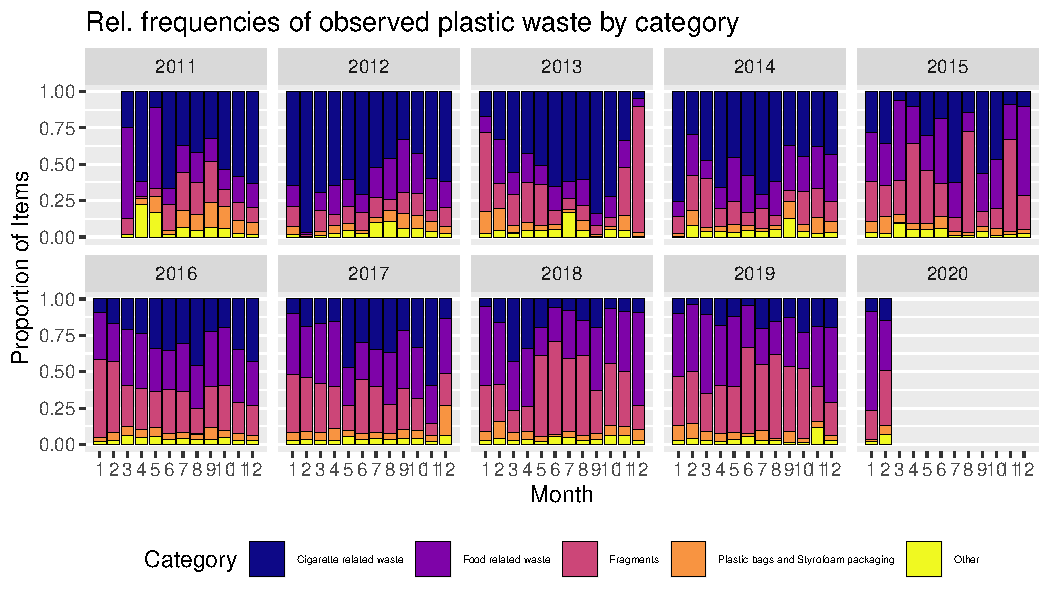
\includegraphics[width=1\linewidth]{figure/unnamed-chunk-8-1} 
\begin{kframe}\begin{alltt}
    \hlcom{#scale_fill_viridis_d(option = "magma")}

\hlcom{#ggsave("plots/pastic_debris_plot.png", width = 40, height = 20, units = "cm")}
\end{alltt}
\end{kframe}
\end{knitrout}
\caption {Debris by categorisation}
\label{figE}
\end {center}
\end {figure}




\hl{Adjust legend text size in annotated code below. - Stuart}
\begin{figure}[H] %start a figure
\begin{center}
\begin{knitrout}\small
\definecolor{shadecolor}{rgb}{0.969, 0.969, 0.969}\color{fgcolor}\begin{kframe}
\begin{alltt}
\hlcom{# all cigarette related waste: 1, 4, 6, 22}
\hlcom{# Food related waste: 3, 2,7,9,10, 17, 23, 11}
\hlcom{# Non food related waste: 8, 14, 15, 16, 18, 19, 21, 20}
\hlcom{# Plastic bags and Styrofoam packaging:12, 13}
\hlcom{# Fragments: 5, 23, 24,25}

\hlstd{recategorise} \hlkwb{<-} \hlkwa{function}\hlstd{(}\hlkwc{x}\hlstd{)\{}
  \hlstd{out} \hlkwb{=} \hlstr{""}
  \hlkwa{if}\hlstd{(x} \hlopt \hlkwd{c}\hlstd{(}\hlnum{1}\hlstd{,}\hlnum{4}\hlstd{,}\hlnum{6}\hlstd{,}\hlnum{22}\hlstd{))\{out} \hlkwb{=} \hlstr{"Cigarette related waste"}\hlstd{\}}
  \hlkwa{if}\hlstd{(x} \hlopt \hlkwd{c}\hlstd{(}\hlnum{2}\hlstd{,}\hlnum{3}\hlstd{,}\hlnum{7}\hlstd{,}\hlnum{9}\hlstd{,}\hlnum{10}\hlstd{,}\hlnum{17}\hlstd{,}\hlnum{23}\hlstd{,}\hlnum{11}\hlstd{)) out} \hlkwb{=} \hlstr{"Food related waste"}
  \hlkwa{if}\hlstd{(x} \hlopt \hlkwd{c}\hlstd{(}\hlnum{8}\hlstd{,}\hlnum{14}\hlstd{,}\hlnum{15}\hlstd{,}\hlnum{16}\hlstd{,}\hlnum{18}\hlstd{,}\hlnum{19}\hlstd{,}\hlnum{21}\hlstd{,}\hlnum{20}\hlstd{)) out} \hlkwb{=} \hlstr{"Other"}
  \hlkwa{if}\hlstd{(x} \hlopt \hlkwd{c}\hlstd{(}\hlnum{12}\hlstd{,}\hlnum{13}\hlstd{)) out} \hlkwb{=} \hlstr{"Plastic bags and Styrofoam packaging"}
  \hlkwa{if}\hlstd{(x} \hlopt \hlkwd{c}\hlstd{(}\hlnum{5}\hlstd{,}\hlnum{23}\hlstd{,}\hlnum{24}\hlstd{,}\hlnum{25}\hlstd{)) out} \hlkwb{=} \hlstr{"Fragments"}
  \hlkwa{if}\hlstd{(out} \hlopt{==} \hlstr{""}\hlstd{)} \hlkwd{stop}\hlstd{(}\hlkwd{paste}\hlstd{(}\hlstr{"Error in recategorise:"}\hlstd{, x))}
  \hlkwd{return}\hlstd{(out)}
\hlstd{\}}

\hlstd{plastic_types} \hlkwb{<-} \hlstd{data} \hlopt
  \hlkwd{filter}\hlstd{(`Material Description`} \hlopt{==} \hlstr{"PLASTIC"}\hlstd{)} \hlopt
  \hlkwd{select}\hlstd{(ItemName, ItemID)} \hlopt
  \hlkwd{distinct}\hlstd{()} \hlopt
  \hlkwd{mutate}\hlstd{(}\hlkwc{label} \hlstd{=} \hlnum{1}\hlopt{:}\hlkwd{n}\hlstd{())} \hlopt
  \hlkwd{mutate}\hlstd{(}\hlkwc{category} \hlstd{= purrr}\hlopt{::}\hlkwd{map}\hlstd{(label, recategorise))} \hlopt
  \hlkwd{mutate}\hlstd{(}\hlkwc{category} \hlstd{=} \hlkwd{as_factor}\hlstd{(}\hlkwd{as.character}\hlstd{(category)))} \hlopt
  \hlkwd{select}\hlstd{(ItemID, category)}


\hlstd{plastic} \hlkwb{<-} \hlstd{data} \hlopt
  \hlkwd{filter}\hlstd{(`Material Description`} \hlopt{==} \hlstr{"PLASTIC"}\hlstd{)} \hlopt
  \hlkwd{full_join}\hlstd{(plastic_types,} \hlkwc{by} \hlstd{=} \hlstr{"ItemID"}\hlstd{)}

\hlstd{ordered_levels} \hlkwb{<-} \hlstd{plastic} \hlopt
  \hlkwd{group_by}\hlstd{(category)} \hlopt
  \hlkwd{summarise}\hlstd{(}\hlkwc{totObs} \hlstd{=} \hlkwd{sum}\hlstd{(Quantity))} \hlopt
  \hlkwd{ungroup}\hlstd{()} \hlopt
  \hlkwd{arrange}\hlstd{(}\hlkwd{desc}\hlstd{(totObs))} \hlopt
  \hlkwd{select}\hlstd{(category)} \hlopt
  \hlstd{category}
\hlstd{plastic}\hlopt{$}\hlstd{category} \hlkwb{<-} \hlkwd{factor}\hlstd{(plastic}\hlopt{$}\hlstd{category,} \hlkwc{levels} \hlstd{= ordered_levels)}
\hlkwd{rm}\hlstd{(ordered_levels)}


\hlstd{plastic} \hlopt
  \hlkwd{mutate}\hlstd{(}\hlkwc{month} \hlstd{=} \hlkwd{month}\hlstd{(Time,} \hlkwc{label} \hlstd{=} \hlnum{FALSE}\hlstd{),}
         \hlkwc{year} \hlstd{=} \hlkwd{as.integer}\hlstd{(}\hlkwd{year}\hlstd{(Time)))} \hlopt
  \hlkwd{filter}\hlstd{(year} \hlopt{>} \hlnum{2010}\hlstd{)} \hlopt
  \hlkwd{group_by}\hlstd{(month, year, category)} \hlopt
  \hlkwd{summarise}\hlstd{(}\hlkwc{`Total Quantity`} \hlstd{=} \hlkwd{sum}\hlstd{(Quantity))} \hlopt
  \hlkwd{ggplot}\hlstd{(}\hlkwd{aes}\hlstd{(}\hlkwc{x} \hlstd{= month,} \hlkwc{y} \hlstd{= `Total Quantity`,} \hlkwc{fill} \hlstd{= category))} \hlopt{+}
    \hlkwd{geom_col}\hlstd{(}\hlkwc{colour} \hlstd{=} \hlstr{"black"}\hlstd{,} \hlkwc{size} \hlstd{=} \hlnum{0.2}\hlstd{,} \hlkwc{position} \hlstd{=} \hlstr{"fill"}\hlstd{)} \hlopt{+}
    \hlkwd{facet_wrap}\hlstd{(}\hlopt{~}\hlstd{year,} \hlkwc{nrow} \hlstd{=} \hlnum{2}\hlstd{)} \hlopt{+}
    \hlkwd{scale_fill_viridis}\hlstd{(}\hlkwc{discrete} \hlstd{=} \hlnum{TRUE}\hlstd{,} \hlkwc{option} \hlstd{=} \hlstr{"plasma"}\hlstd{)} \hlopt{+}
    \hlkwd{xlab}\hlstd{(}\hlstr{"Month"}\hlstd{)} \hlopt{+}
    \hlkwd{ylab}\hlstd{(}\hlstr{"Proportion of Items"}\hlstd{)} \hlopt{+}
    \hlkwd{ggtitle}\hlstd{(}\hlstr{"Rel. frequencies of observed plastic waste by category"}\hlstd{)} \hlopt{+}
    \hlkwd{scale_x_continuous}\hlstd{(}\hlkwc{breaks} \hlstd{=} \hlnum{1}\hlopt{:}\hlnum{12}\hlstd{)} \hlopt{+}
    \hlkwd{theme}\hlstd{(}\hlkwc{panel.grid.major.x} \hlstd{=} \hlkwd{element_blank}\hlstd{(),}
          \hlkwc{panel.grid.minor.x} \hlstd{=} \hlkwd{element_blank}\hlstd{(),}
          \hlkwc{legend.position} \hlstd{=} \hlstr{"bottom"}\hlstd{,}
          \hlkwc{legend.text}\hlstd{=}\hlkwd{element_text}\hlstd{(}\hlkwc{size}\hlstd{=}\hlnum{5}\hlstd{))} \hlopt{+} \hlcom{# --- Change legend text size here! ---}
    \hlkwd{guides}\hlstd{(}\hlkwc{fill}\hlstd{=}\hlkwd{guide_legend}\hlstd{(}\hlkwc{title}\hlstd{=}\hlstr{"Category"}\hlstd{))}
\end{alltt}
\end{kframe}
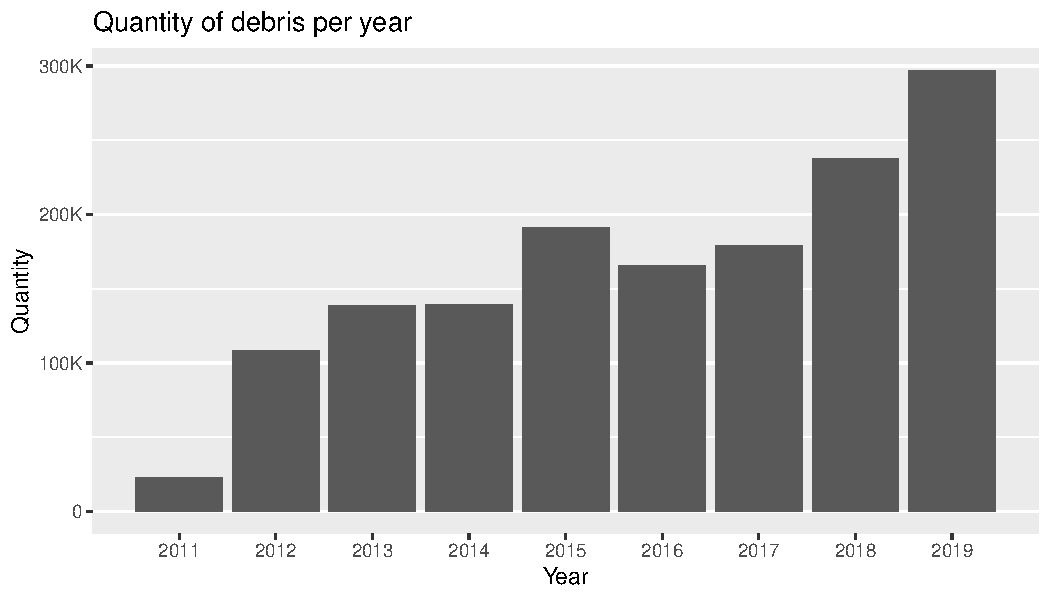
\includegraphics[width=1\linewidth]{figure/unnamed-chunk-9-1} 
\begin{kframe}\begin{alltt}
\hlcom{#ggsave("plots/pastic_debris_plot_recategorised.png", width = 40, height = 20, units = "cm")}
\end{alltt}
\end{kframe}
\end{knitrout}
\caption {Recategorisation by year. Colour scale ordered by ranking of total observed quantity.}
\label{figB}
\end {center}
\end {figure}



\pagebreak
\section{Exploration}

Here we describe the things we found... 

\subsection{Proportion Trends}
How pollutant proportions change over time.\\
\\
Cigarette butts proportions and raw counts decrease over time: possibly less people smoking, or moving to vaping\\
\\
General pollution count going down over time?\\
\\
Old pollutants fall away (cigarette butts) but new ones are introduced\\
\\
Question: Are observed plastic item proportions time invariant?\\
\\

\begin{figure}[H] %start a figure
\begin{center}
\begin{knitrout}\small
\definecolor{shadecolor}{rgb}{0.969, 0.969, 0.969}\color{fgcolor}\begin{kframe}
\begin{alltt}
\hlcom{#Linechart quantity of debris per year}
\hlstd{data} \hlopt
  \hlkwd{mutate}\hlstd{(}\hlkwc{year} \hlstd{=} \hlkwd{year}\hlstd{(Time))} \hlopt
  \hlkwd{filter}\hlstd{(year} \hlopt{>} \hlnum{2010}\hlstd{, year} \hlopt{<} \hlnum{2020}\hlstd{)} \hlopt
  \hlkwd{group_by}\hlstd{(year)} \hlopt
  \hlkwd{summarise}\hlstd{(}\hlkwc{quan} \hlstd{=} \hlkwd{sum}\hlstd{(Quantity))} \hlopt
  \hlkwd{ggplot}\hlstd{(}\hlkwd{aes}\hlstd{(}\hlkwc{x} \hlstd{= year,} \hlkwc{y} \hlstd{= quan))} \hlopt{+}
    \hlkwd{geom_col}\hlstd{()} \hlopt{+}
    \hlkwd{scale_x_continuous}\hlstd{(}\hlkwc{breaks} \hlstd{=} \hlnum{2011}\hlopt{:}\hlnum{2019}\hlstd{)} \hlopt{+}
    \hlkwd{xlab}\hlstd{(}\hlstr{"Year"}\hlstd{)} \hlopt{+}
    \hlkwd{ylab}\hlstd{(}\hlstr{"Quantity"}\hlstd{)} \hlopt{+}
    \hlkwd{ggtitle}\hlstd{(}\hlstr{"Quantity of debris per year"}\hlstd{)} \hlopt{+}
    \hlkwd{theme}\hlstd{(}\hlkwc{panel.grid.major.x} \hlstd{=} \hlkwd{element_blank}\hlstd{(),}
          \hlkwc{panel.grid.minor.x} \hlstd{=} \hlkwd{element_blank}\hlstd{())} \hlopt{+}
    \hlkwd{scale_y_continuous}\hlstd{(}\hlkwc{labels} \hlstd{= scales}\hlopt{::}\hlkwd{label_number_si}\hlstd{(}\hlkwc{accuracy} \hlstd{=} \hlnum{1}\hlstd{))}
\end{alltt}
\end{kframe}
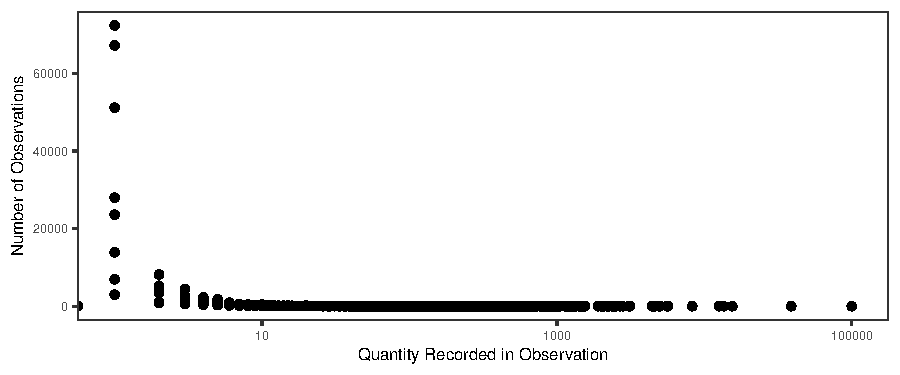
\includegraphics[width=1\linewidth]{figure/unnamed-chunk-10-1} 
\begin{kframe}\begin{alltt}
\hlcom{#ggsave("plots/observations.png")}
\end{alltt}
\end{kframe}
\end{knitrout}
\caption {Trend of debris observered}
\label{figD}
\end {center}
\end {figure}


\begin{figure}[H] %start a figure
\begin{center}
\begin{knitrout}\small
\definecolor{shadecolor}{rgb}{0.969, 0.969, 0.969}\color{fgcolor}\begin{kframe}
\begin{alltt}
\hlcom{#Histogram of observations: Total v Plastic}
\hlstd{data} \hlopt
  \hlkwd{mutate}\hlstd{(}\hlkwc{Type} \hlstd{=} \hlkwd{if_else}\hlstd{(`Material Description`} \hlopt{==} \hlstr{"PLASTIC"}\hlstd{,} \hlstr{"Plastic"}\hlstd{,} \hlstr{"Other"}\hlstd{),}
         \hlkwc{months} \hlstd{=} \hlkwd{floor_date}\hlstd{(Time,} \hlstr{'month'}\hlstd{))} \hlopt
  \hlkwd{group_by}\hlstd{(months, Type)} \hlopt
  \hlkwd{summarize}\hlstd{(}\hlkwc{`Number of observations`} \hlstd{=} \hlkwd{n}\hlstd{())} \hlopt
  \hlkwd{ggplot}\hlstd{(}\hlkwd{aes}\hlstd{(}\hlkwc{x} \hlstd{= months,} \hlkwc{y} \hlstd{= `Number of observations`))} \hlopt{+}
    \hlkwd{geom_area}\hlstd{(}\hlkwd{aes}\hlstd{(}\hlkwc{fill} \hlstd{= Type))} \hlopt{+}
    \hlkwd{theme}\hlstd{(}\hlkwc{legend.position} \hlstd{=} \hlstr{"bottom"}\hlstd{)}
\end{alltt}
\end{kframe}
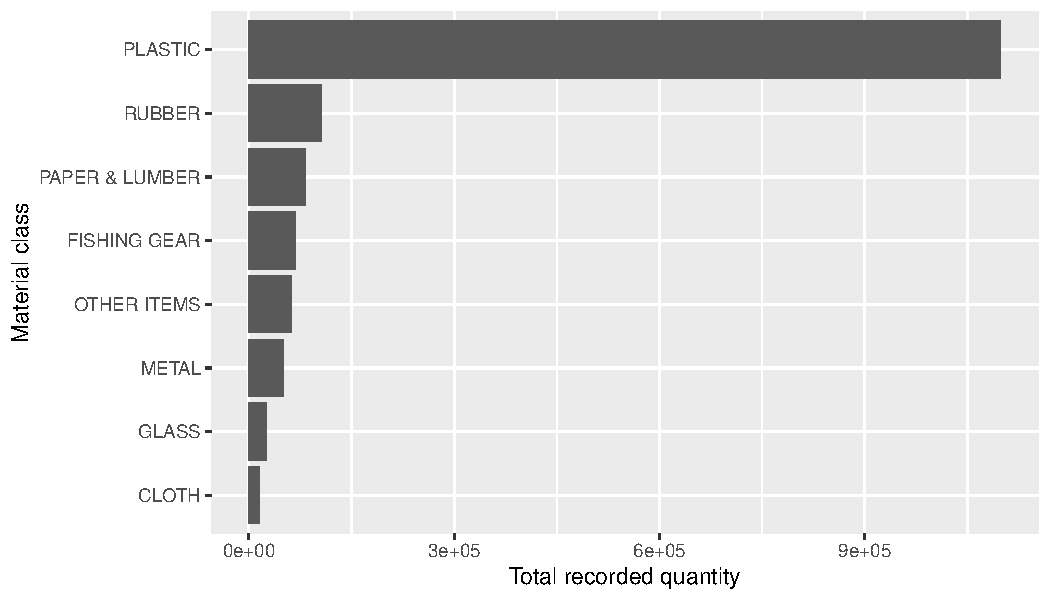
\includegraphics[width=1\linewidth]{figure/unnamed-chunk-11-1} 
\begin{kframe}\begin{alltt}
  \hlcom{# ggplot() +}
  \hlcom{# geom_histogram(aes(x = Time))}
\end{alltt}
\end{kframe}
\end{knitrout}
\caption {Observations of plastic debris v all debris}
\label{figF}
\end {center}
\end {figure}


\subsection {Distribution of observed debris:}

MaterialQuantities\\

\begin{figure}[H] %start a figure
\begin{center}
\begin{knitrout}\small
\definecolor{shadecolor}{rgb}{0.969, 0.969, 0.969}\color{fgcolor}\begin{kframe}
\begin{alltt}
\hlstd{data} \hlopt \hlkwd{select}\hlstd{(Quantity,Description,`Material Description`)} \hlopt
  \hlkwd{group_by}\hlstd{(`Material Description`)} \hlopt
  \hlkwd{summarise}\hlstd{(}\hlkwc{Quantity} \hlstd{=} \hlkwd{sum}\hlstd{(Quantity))} \hlopt

  \hlkwd{ggplot}\hlstd{(}\hlkwd{aes}\hlstd{(}\hlkwc{x} \hlstd{=} \hlkwd{reorder}\hlstd{(`Material Description`, Quantity),} \hlkwc{y} \hlstd{= Quantity))} \hlopt{+}
    \hlkwd{geom_col}\hlstd{()} \hlopt{+}
    \hlkwd{ylab}\hlstd{(}\hlstr{"Total recorded quantity"}\hlstd{)} \hlopt{+}
    \hlkwd{xlab}\hlstd{(}\hlstr{"Material class"}\hlstd{)} \hlopt{+}
    \hlkwd{coord_flip}\hlstd{()}
\end{alltt}
\end{kframe}
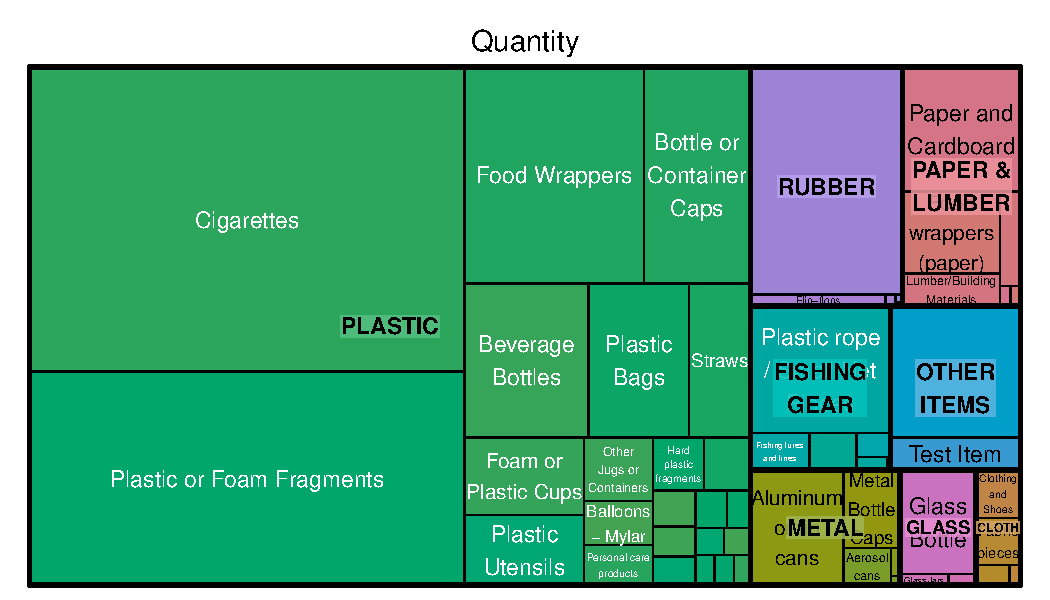
\includegraphics[width=1\linewidth]{figure/unnamed-chunk-12-1} 

\end{knitrout}
\caption {Material Quantities}
\label{figC}
\end {center}
\end {figure}

So the most populated material class is Plastic. Note that this does not necessarily mean that plastic is the largest quantity of debris, just that the individual number of items categorised is largest.

A tree map of material quantities:
\begin{figure}[H] %start a figure
\begin{center}
\begin{knitrout}\small
\definecolor{shadecolor}{rgb}{0.969, 0.969, 0.969}\color{fgcolor}\begin{kframe}
\begin{alltt}
\hlcom{#treemap of debris categories}
\hlcom{#png("plots/treemap.png")}
\hlstd{data} \hlopt
  \hlkwd{select}\hlstd{(`Material Description`, ItemName, Quantity)} \hlopt
  \hlkwd{group_by}\hlstd{(`Material Description`, ItemName)} \hlopt
  \hlkwd{summarise}\hlstd{(}\hlkwc{Quantity} \hlstd{=} \hlkwd{sum}\hlstd{(Quantity))} \hlopt
  \hlkwd{treemap}\hlstd{(}\hlkwc{index} \hlstd{=} \hlkwd{c}\hlstd{(}\hlstr{"Material Description"}\hlstd{,} \hlstr{"ItemName"}\hlstd{),}
          \hlkwc{vSize} \hlstd{=} \hlstr{"Quantity"}\hlstd{,} \hlkwc{draw} \hlstd{=} \hlnum{TRUE}\hlstd{)} \hlkwb{->} \hlstd{tm}
\end{alltt}
\end{kframe}
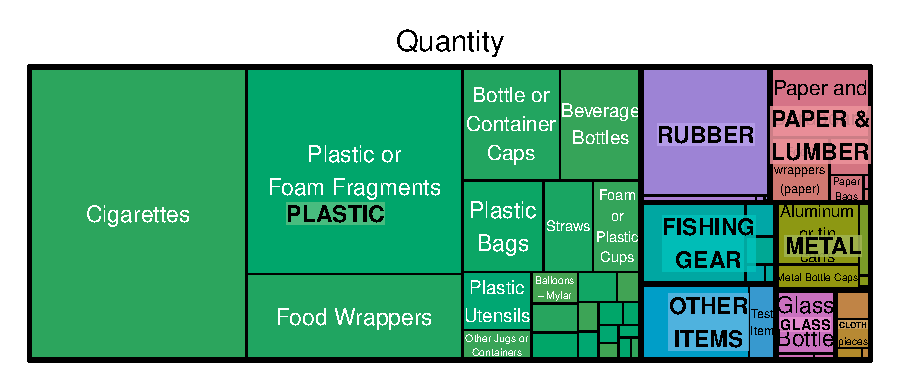
\includegraphics[width=1\linewidth]{figure/unnamed-chunk-13-1} 
\begin{kframe}\begin{alltt}
\hlcom{#tm}
\hlcom{#dev.off()}
\hlcom{#save.image(file = "plots/treemap.png")}
\end{alltt}
\end{kframe}
\end{knitrout}
\caption {Debris categorisation}
\label{figI}
\end {center}
\end {figure}

Cigarettes are the most common item recorded as seen in. %Figure~\ref{figI}
Perhaps some of the debris is not actually from the sea, but rather from people littering by the coastline? Does debris littered on the coastline end up in the oceans?

\hl{This is a great chart, but not the best to support the statement that cigarettes is most popular - a column or bar chart here will be much better (area charts are not as effective as charts you can level-compare), potentially use proportions or data labels to further drive the point that it IS the largest. Treemap suggest moving back into pre-processing section.}


\begin{figure}[H] %start a figure
\begin{center}
\begin{knitrout}\small
\definecolor{shadecolor}{rgb}{0.969, 0.969, 0.969}\color{fgcolor}\begin{kframe}
\begin{alltt}
\hlcom{#bar of debris categories}
\hlstd{data} \hlopt
  \hlkwd{select}\hlstd{(`Material Description`, ItemName, Quantity)} \hlopt
  \hlkwd{group_by}\hlstd{(`Material Description`, ItemName)} \hlopt
  \hlkwd{summarise}\hlstd{(}\hlkwc{Quantity} \hlstd{=} \hlkwd{sum}\hlstd{(Quantity))} \hlopt
  \hlkwd{ggplot}\hlstd{(}\hlkwd{aes}\hlstd{(}\hlkwc{x}\hlstd{=}\hlkwd{reorder}\hlstd{(`ItemName`,} \hlopt{-}\hlstd{Quantity),} \hlkwc{y}\hlstd{=Quantity,} \hlkwc{fill}\hlstd{=`Material Description`))} \hlopt{+}
  \hlkwd{geom_bar}\hlstd{(}\hlkwc{stat}\hlstd{=}\hlstr{"identity"}\hlstd{)} \hlopt{+}
  \hlkwd{ggtitle}\hlstd{(}\hlstr{"Debris Categorisation"}\hlstd{)} \hlopt{+}
  \hlkwd{xlab}\hlstd{(}\hlstr{"Debris"}\hlstd{)} \hlopt{+}
  \hlkwd{ylab}\hlstd{(}\hlstr{""}\hlstd{)} \hlopt{+}
  \hlcom{#coord_flip() +}
  \hlkwd{theme}\hlstd{(}\hlkwc{text} \hlstd{=} \hlkwd{element_text}\hlstd{(}\hlkwc{size}\hlstd{=}\hlnum{8}\hlstd{),}
        \hlkwc{axis.text.x}\hlstd{=}\hlkwd{element_text}\hlstd{(}\hlkwc{angle}\hlstd{=}\hlnum{90}\hlstd{,} \hlkwc{hjust}\hlstd{=}\hlnum{1}\hlstd{),}
        \hlkwc{plot.title} \hlstd{=} \hlkwd{element_text}\hlstd{(}\hlkwc{size}\hlstd{=}\hlnum{10}\hlstd{),}
        \hlkwc{legend.text}\hlstd{=}\hlkwd{element_text}\hlstd{(}\hlkwc{size}\hlstd{=}\hlnum{5}\hlstd{),}
        \hlkwc{legend.position} \hlstd{=} \hlstr{"bottom"}\hlstd{)}
\end{alltt}
\end{kframe}
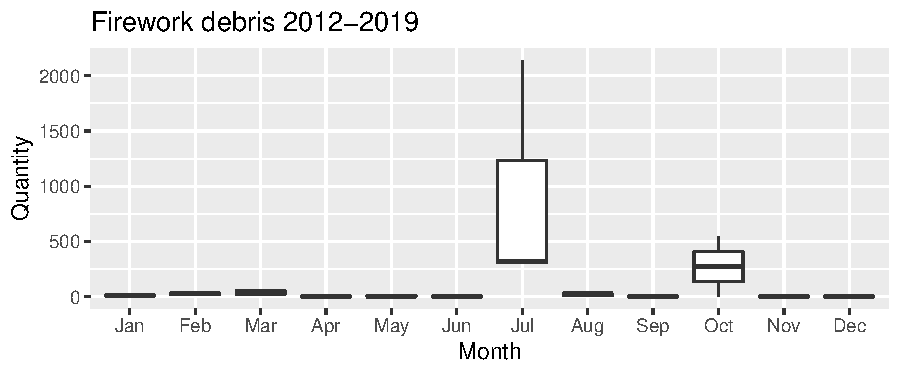
\includegraphics[width=1\linewidth]{figure/unnamed-chunk-14-1} 
\begin{kframe}\begin{alltt}
  \hlcom{#treemap(index = c("Material Description", "ItemName"),}
  \hlcom{#        vSize = "Quantity", draw = TRUE) -> tm}
\end{alltt}
\end{kframe}
\end{knitrout}
\caption {Debris categorisation}
\label{figI2}
\end {center}
\end {figure}

\hl{maybe make this top 10 or 15 items.}


\subsection{Event-Driven Pollution}

Fireworks found in July and North-America only: possibly 4th July celebrations\\
4th July and Firework link? (Karen's Idea)\\

\begin{figure}[H] %start a figure
\begin{center}
\begin{knitrout}\small
\definecolor{shadecolor}{rgb}{0.969, 0.969, 0.969}\color{fgcolor}\begin{kframe}
\begin{alltt}
\hlcom{#Boxplot of fireworks distribution by month (across all years)}
\hlstd{data} \hlopt
  \hlkwd{filter}\hlstd{(`Material Description`} \hlopt{==} \hlstr{"PLASTIC"}\hlstd{,}
         \hlstd{ItemName} \hlopt \hlkwd{c}\hlstd{(}\hlstr{"Fireworks"}\hlstd{),}
         \hlkwd{year}\hlstd{(Time)} \hlopt{>=} \hlnum{2012}\hlstd{,} \hlkwd{year}\hlstd{(Time)} \hlopt{<=} \hlnum{2019}\hlstd{)} \hlopt
  \hlkwd{mutate}\hlstd{(}\hlkwc{month} \hlstd{=} \hlkwd{month}\hlstd{(Time,} \hlkwc{label} \hlstd{=} \hlnum{TRUE}\hlstd{),}
         \hlkwc{year} \hlstd{=} \hlkwd{as.integer}\hlstd{(}\hlkwd{year}\hlstd{(Time)))} \hlopt
  \hlkwd{group_by}\hlstd{(month, year)} \hlopt
  \hlkwd{summarise}\hlstd{(}\hlkwc{quantity} \hlstd{=} \hlkwd{sum}\hlstd{(Quantity))} \hlopt
  \hlkwd{ggplot}\hlstd{()} \hlopt{+}
    \hlkwd{geom_boxplot}\hlstd{(}\hlkwd{aes}\hlstd{(}\hlkwc{x} \hlstd{= month,} \hlkwc{y} \hlstd{= quantity))} \hlopt{+}
    \hlkwd{xlab}\hlstd{(}\hlstr{"Month"}\hlstd{)} \hlopt{+}
    \hlkwd{ylab}\hlstd{(}\hlstr{"Quantity"}\hlstd{)} \hlopt{+}
    \hlkwd{ggtitle}\hlstd{(}\hlstr{"Firework debris 2012-2019"}\hlstd{)}
\end{alltt}
\end{kframe}
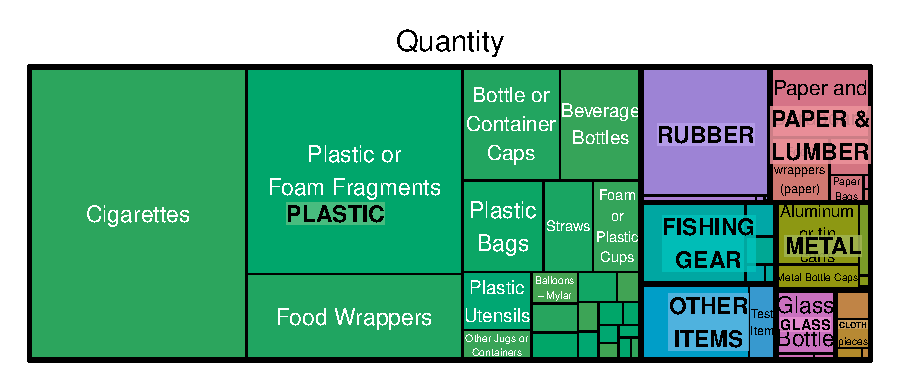
\includegraphics[width=1\linewidth]{figure/unnamed-chunk-15-1} 
\begin{kframe}\begin{alltt}
\hlcom{#ggsave("plots/fireworks.png")}
\end{alltt}
\end{kframe}
\end{knitrout}

\caption {Boxplot of fireworks distribution by month, across all years}
\label{figA}
\end {center}
\end {figure}





\subsection{Location-Driven Pollution}

Rubber found in Indoneasia only: possibly a recording bias.\\

Certain classes are found in certain regions only: not because they don't exist elsewhere but because of recording bias focus in those areas\\

We have locational data, so lets check for any geographical observation bias.
\begin{knitrout}\small
\definecolor{shadecolor}{rgb}{0.969, 0.969, 0.969}\color{fgcolor}\begin{kframe}
\begin{alltt}
\hlstd{world} \hlkwb{<-} \hlkwd{map_data}\hlstd{(}\hlstr{"world"}\hlstd{)}
\hlstd{data} \hlopt
  \hlkwd{select}\hlstd{(Latitude, Longitude, Quantity, Location, `Material Description`)} \hlopt
  \hlkwd{ggplot}\hlstd{()} \hlopt{+}
    \hlkwd{geom_polygon}\hlstd{(}\hlkwc{data} \hlstd{=} \hlkwd{map_data}\hlstd{(}\hlstr{"world"}\hlstd{),} \hlkwd{aes}\hlstd{(}\hlkwc{x} \hlstd{= long,} \hlkwc{y} \hlstd{= lat,} \hlkwc{group} \hlstd{= group),} \hlkwc{fill} \hlstd{=} \hlstr{"grey"}\hlstd{,} \hlkwc{alpha} \hlstd{=} \hlnum{0.5}\hlstd{)} \hlopt{+}
    \hlkwd{geom_hex}\hlstd{(}\hlkwd{aes}\hlstd{(}\hlkwc{x} \hlstd{= Longitude,} \hlkwc{y} \hlstd{= Latitude),} \hlkwc{bins} \hlstd{=} \hlnum{50}\hlstd{)} \hlopt{+}
    \hlkwd{scale_fill_viridis}\hlstd{(}\hlkwc{trans} \hlstd{=} \hlstr{"log"}\hlstd{,} \hlkwc{breaks} \hlstd{=} \hlkwd{c}\hlstd{(}\hlnum{5}\hlstd{,} \hlnum{50}\hlstd{,} \hlnum{500}\hlstd{,} \hlnum{5000}\hlstd{,} \hlnum{50000}\hlstd{))} \hlopt{+}
    \hlkwd{theme_void}\hlstd{()} \hlopt{+}
    \hlkwd{guides}\hlstd{(}\hlkwc{fill}\hlstd{=}\hlkwd{guide_legend}\hlstd{(}\hlkwc{title}\hlstd{=}\hlstr{"Observations"}\hlstd{))}
\end{alltt}
\end{kframe}
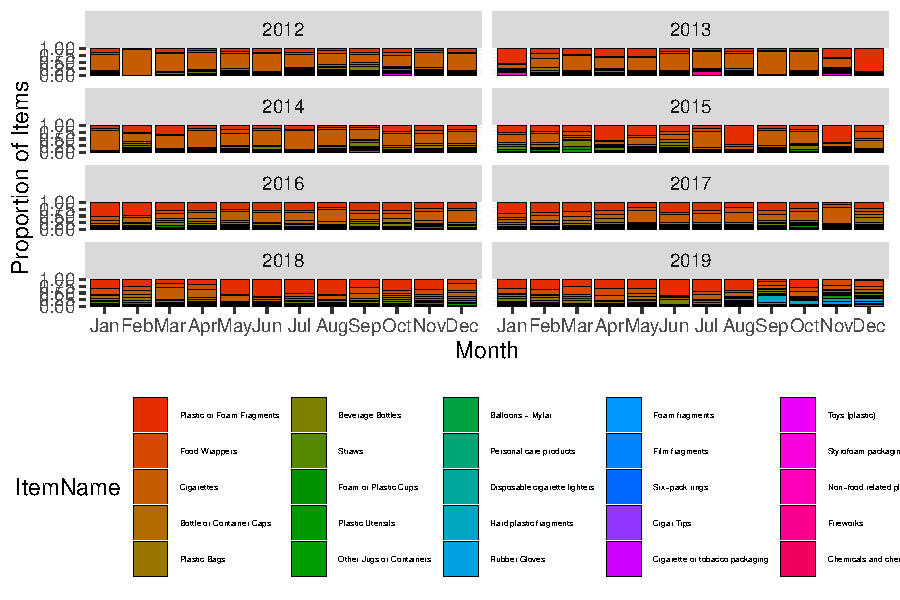
\includegraphics[width=1\linewidth]{figure/unnamed-chunk-16-1} 
\begin{kframe}\begin{alltt}
\hlcom{#ggsave("plots/map.png", width = 20, height = 10, units = "cm")}
\end{alltt}
\end{kframe}
\end{knitrout}

We need to know how reliable the location data is. I'm going to filter for "united kingdom" in the location field and plot the raw coordinates.\\

\begin{figure}[H] %start a figure
\begin{center}

\caption {Longitude and Latitude discrepancies}
\label{figJ}
\end {center}
\end {figure}


Questions\\
Distribution of plastic by location.\\
Are the distributions of plastic fairly constant for the locations with the most observations?\\
\begin{figure}[H] %start a figure
\begin{center}
\begin{knitrout}\small
\definecolor{shadecolor}{rgb}{0.969, 0.969, 0.969}\color{fgcolor}\begin{kframe}
\begin{alltt}
\hlcom{#columnchart of debris locations}
\hlstd{topLocations} \hlkwb{<-} \hlstd{data} \hlopt
  \hlkwd{group_by}\hlstd{(Location)} \hlopt
  \hlkwd{summarise}\hlstd{(}\hlkwc{sumQuantity} \hlstd{=} \hlkwd{sum}\hlstd{(Quantity))} \hlopt
  \hlkwd{arrange}\hlstd{(}\hlkwd{desc}\hlstd{(sumQuantity))} \hlopt
  \hlkwd{top_n}\hlstd{(}\hlnum{5}\hlstd{,sumQuantity)}

\hlstd{data} \hlopt
  \hlkwd{filter}\hlstd{(Location} \hlopt \hlstd{topLocations}\hlopt{$}\hlstd{Location)} \hlopt
  \hlkwd{group_by}\hlstd{(Location, `Material Description`)} \hlopt
  \hlkwd{summarise}\hlstd{(}\hlkwc{sumQuantity} \hlstd{=} \hlkwd{sum}\hlstd{(Quantity))} \hlopt
  \hlkwd{arrange}\hlstd{(}\hlkwd{desc}\hlstd{(sumQuantity))} \hlopt
  \hlkwd{ggplot}\hlstd{(}\hlkwd{aes}\hlstd{(}\hlkwc{x} \hlstd{= `Material Description`,} \hlkwc{y} \hlstd{= sumQuantity,} \hlkwc{fill} \hlstd{= Location))} \hlopt{+}
    \hlkwd{geom_col}\hlstd{()} \hlopt{+} \hlkwd{theme}\hlstd{(}\hlkwc{legend.position} \hlstd{=} \hlstr{'top'}\hlstd{)}
\end{alltt}
\end{kframe}
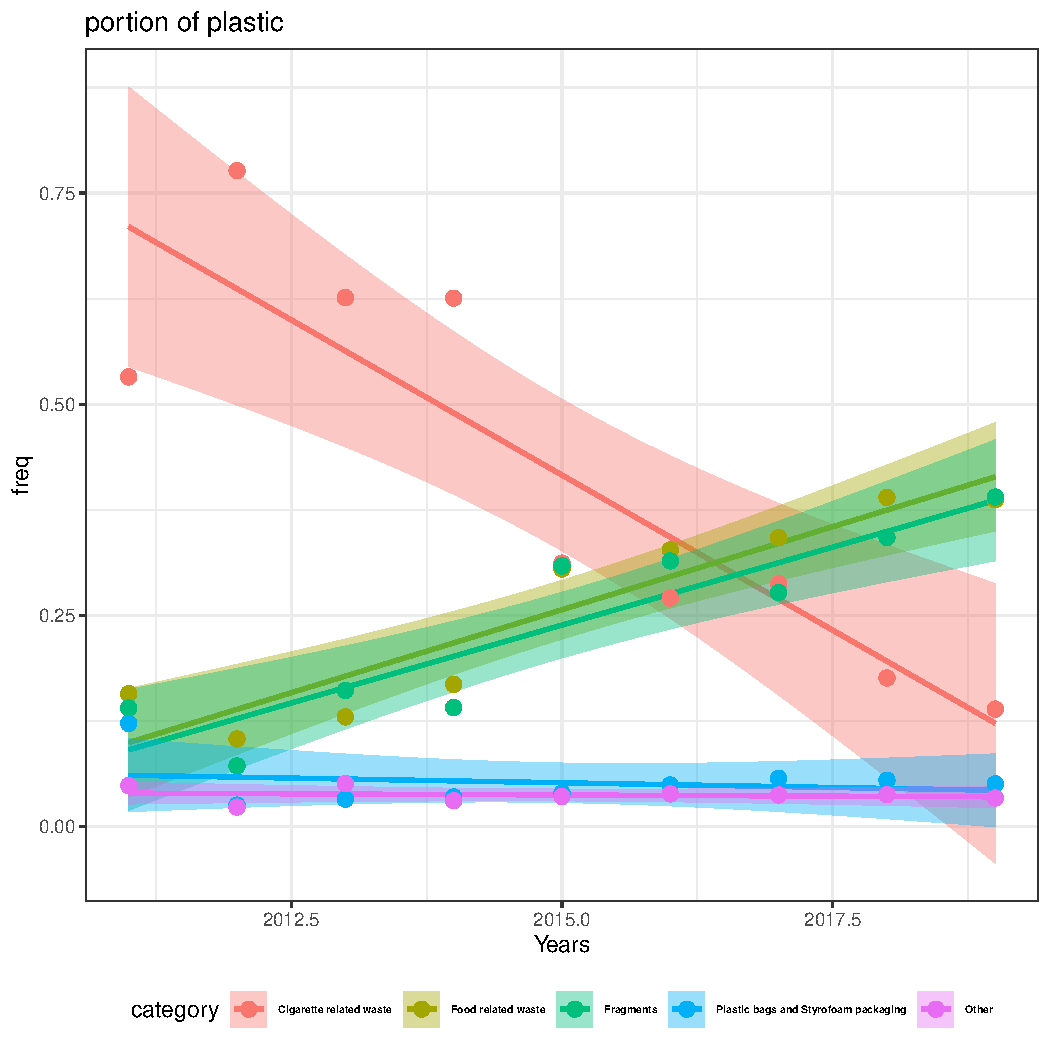
\includegraphics[width=1\linewidth]{figure/unnamed-chunk-18-1} 

\end{knitrout}
\caption {Debris by location}
\label{figG}
\end {center}
\end {figure}
We see that the Location "unknown" has the most plastic... note that this is distinct from "(Missing)", which was our original NA values. Maybe we should merge these.



\subsection{Item Pairing} 
(e.g. are 6-pack beer rings observed at the same time as fireworks? )
\hl{are we going to explore this one?}

\pagebreak
\section{Predictive Modelling}
Given the variability of plastic pollution trends given event-driven and location-driven pollution as explored earlier in this report, the authors of this report built a model to predict the proportion of plastics given Month and Location. This would give more accurate predictions as opposed to a simple linear model accomodating such time factored

\subsection{Description of Model}

Georgios' script
\begin{knitrout}\small
\definecolor{shadecolor}{rgb}{0.969, 0.969, 0.969}\color{fgcolor}\begin{kframe}
\begin{alltt}
\hlstd{plasticN} \hlkwb{<-} \hlstd{plastic} \hlopt
  \hlkwd{mutate}\hlstd{(}\hlkwc{month} \hlstd{=} \hlkwd{month}\hlstd{(Time,} \hlkwc{label} \hlstd{=} \hlnum{FALSE}\hlstd{),} \hlkwc{year} \hlstd{=} \hlkwd{as.integer}\hlstd{(}\hlkwd{year}\hlstd{(Time)))} \hlopt
  \hlkwd{filter}\hlstd{(year} \hlopt{>} \hlnum{2010}\hlstd{)} \hlopt
  \hlkwd{group_by}\hlstd{(year, category, month)} \hlopt
  \hlkwd{summarise}\hlstd{(}\hlkwc{`Total Quantity`} \hlstd{=} \hlkwd{sum}\hlstd{(Quantity))}



\hlcom{####}


\hlstd{df11N} \hlkwb{<-} \hlstd{plasticN}  \hlopt
  \hlkwd{filter}\hlstd{(year} \hlopt{==} \hlnum{2011}\hlstd{)} \hlopt
  \hlkwd{group_by}\hlstd{(year, month)} \hlopt
  \hlkwd{mutate}\hlstd{(}\hlkwc{freq} \hlstd{= `Total Quantity`} \hlopt{/} \hlkwd{sum}\hlstd{(`Total Quantity`))}

\hlstd{df12N} \hlkwb{<-} \hlstd{plasticN}  \hlopt
  \hlkwd{filter}\hlstd{(year} \hlopt{==} \hlnum{2012}\hlstd{)} \hlopt
  \hlkwd{group_by}\hlstd{(year, month)} \hlopt
  \hlkwd{mutate}\hlstd{(}\hlkwc{freq} \hlstd{= `Total Quantity`} \hlopt{/} \hlkwd{sum}\hlstd{(`Total Quantity`))}


\hlstd{df13N} \hlkwb{<-} \hlstd{plasticN}  \hlopt
  \hlkwd{filter}\hlstd{(year} \hlopt{==} \hlnum{2013}\hlstd{)} \hlopt
  \hlkwd{group_by}\hlstd{(year, month)} \hlopt
  \hlkwd{mutate}\hlstd{(}\hlkwc{freq} \hlstd{= `Total Quantity`} \hlopt{/} \hlkwd{sum}\hlstd{(`Total Quantity`))}


\hlstd{df14N} \hlkwb{<-} \hlstd{plasticN}  \hlopt
  \hlkwd{filter}\hlstd{(year} \hlopt{==} \hlnum{2014}\hlstd{)} \hlopt
  \hlkwd{group_by}\hlstd{(year, month)} \hlopt
  \hlkwd{mutate}\hlstd{(}\hlkwc{freq} \hlstd{= `Total Quantity`} \hlopt{/} \hlkwd{sum}\hlstd{(`Total Quantity`))}

\hlstd{df15N} \hlkwb{<-} \hlstd{plasticN}  \hlopt
  \hlkwd{filter}\hlstd{(year} \hlopt{==} \hlnum{2015}\hlstd{)} \hlopt
  \hlkwd{group_by}\hlstd{(year, month)} \hlopt
  \hlkwd{mutate}\hlstd{(}\hlkwc{freq} \hlstd{= `Total Quantity`} \hlopt{/} \hlkwd{sum}\hlstd{(`Total Quantity`))}


\hlstd{df16N} \hlkwb{<-} \hlstd{plasticN}  \hlopt
  \hlkwd{filter}\hlstd{(year} \hlopt{==} \hlnum{2016}\hlstd{)} \hlopt
  \hlkwd{group_by}\hlstd{(year, month)} \hlopt
  \hlkwd{mutate}\hlstd{(}\hlkwc{freq} \hlstd{= `Total Quantity`} \hlopt{/} \hlkwd{sum}\hlstd{(`Total Quantity`))}



\hlstd{df17N} \hlkwb{<-} \hlstd{plasticN}  \hlopt
  \hlkwd{filter}\hlstd{(year} \hlopt{==} \hlnum{2017}\hlstd{)} \hlopt
  \hlkwd{group_by}\hlstd{(year, month)} \hlopt
  \hlkwd{mutate}\hlstd{(}\hlkwc{freq} \hlstd{= `Total Quantity`} \hlopt{/} \hlkwd{sum}\hlstd{(`Total Quantity`))}


\hlstd{df18N} \hlkwb{<-} \hlstd{plasticN}  \hlopt
  \hlkwd{filter}\hlstd{(year} \hlopt{==} \hlnum{2018}\hlstd{)} \hlopt
  \hlkwd{group_by}\hlstd{(year, month)} \hlopt
  \hlkwd{mutate}\hlstd{(}\hlkwc{freq} \hlstd{= `Total Quantity`} \hlopt{/} \hlkwd{sum}\hlstd{(`Total Quantity`))}

\hlstd{df19N} \hlkwb{<-} \hlstd{plasticN}  \hlopt
  \hlkwd{filter}\hlstd{(year} \hlopt{==} \hlnum{2019}\hlstd{)} \hlopt
  \hlkwd{group_by}\hlstd{(year, month)} \hlopt
  \hlkwd{mutate}\hlstd{(}\hlkwc{freq} \hlstd{= `Total Quantity`} \hlopt{/} \hlkwd{sum}\hlstd{(`Total Quantity`))}


\hlstd{dfTotN} \hlkwb{<-} \hlkwd{rbind}\hlstd{(df11N, df12N, df13N, df14N, df15N, df16N, df17N, df18N, df19N)}
\end{alltt}
\end{kframe}
\end{knitrout}

\begin{figure}[H] %start a figure
\begin{center}
\begin{knitrout}\small
\definecolor{shadecolor}{rgb}{0.969, 0.969, 0.969}\color{fgcolor}\begin{kframe}
\begin{alltt}
\hlcom{# plot for observing the data}
\hlstd{(time_plotfr2N} \hlkwb{<-} \hlkwd{ggplot}\hlstd{(dfTotN,} \hlkwd{aes}\hlstd{(}\hlkwc{x} \hlstd{= year,} \hlkwc{y} \hlstd{= freq,} \hlkwc{color}\hlstd{=category,} \hlkwc{fill} \hlstd{= category))} \hlopt{+}
  \hlkwd{geom_smooth}\hlstd{(}\hlkwc{method}\hlstd{=}\hlstr{"lm"}\hlstd{,} \hlkwc{level}\hlstd{=}\hlnum{0.95}\hlstd{)} \hlopt{+}
  \hlkwd{theme_bw}\hlstd{()} \hlopt{+}
  \hlkwd{xlab}\hlstd{(}\hlstr{"Years"}\hlstd{)} \hlopt{+}
  \hlkwd{ylab}\hlstd{(}\hlstr{"relative frequency"}\hlstd{)} \hlopt{+}
  \hlkwd{ggtitle}\hlstd{(}\hlstr{"portion of plastic"}\hlstd{)} \hlopt{+}
  \hlkwd{expand_limits}\hlstd{(}\hlkwc{y}\hlstd{=}\hlnum{0}\hlstd{)} \hlopt{+}
  \hlkwd{scale_y_continuous}\hlstd{()} \hlopt{+}
  \hlkwd{scale_x_continuous}\hlstd{()}\hlopt{+}
  \hlkwd{theme}\hlstd{(}\hlkwc{legend.position}\hlstd{=}\hlstr{"bottom"}\hlstd{)}\hlopt{+}
  \hlkwd{theme}\hlstd{(}\hlkwc{legend.text} \hlstd{=} \hlkwd{element_text}\hlstd{(}\hlkwc{size}\hlstd{=}\hlnum{5}\hlstd{,} \hlkwc{face}\hlstd{=}\hlstr{"bold"}\hlstd{)))}
\end{alltt}
\end{kframe}
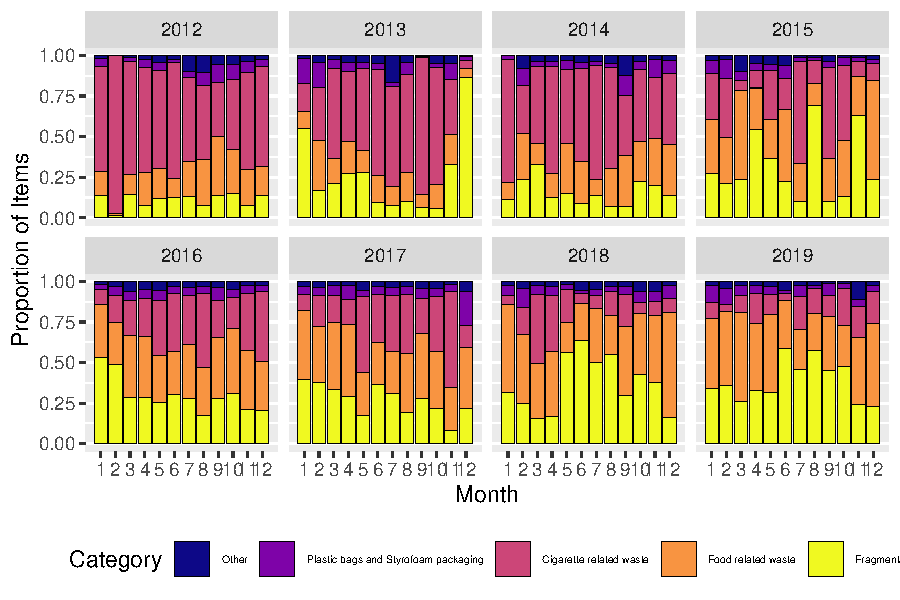
\includegraphics[width=1\linewidth]{figure/unnamed-chunk-20-1} 

\end{knitrout}
\caption {Some sort of caption here}
\label{figG1}
\end {center}
\end {figure}

\begin{knitrout}\small
\definecolor{shadecolor}{rgb}{0.969, 0.969, 0.969}\color{fgcolor}\begin{kframe}
\begin{alltt}
\hlcom{#1/4/20}
\hlcom{### MODELING with new categorisation}


\hlcom{# create train and test set}
\hlstd{n} \hlkwb{<-} \hlkwd{nrow}\hlstd{(dfTotN)}  \hlcom{# Number of observations}
\hlstd{ntrain} \hlkwb{<-} \hlkwd{round}\hlstd{(n}\hlopt{*}\hlnum{0.75}\hlstd{)}  \hlcom{# 75% for training set}
\hlkwd{set.seed}\hlstd{(}\hlnum{314}\hlstd{)}    \hlcom{# Set seed for reproducible results}
\hlstd{tindex} \hlkwb{<-} \hlkwd{sample}\hlstd{(n, ntrain)}   \hlcom{# Create a random index}
\hlstd{train_dfTotN} \hlkwb{<-} \hlstd{dfTotN[tindex,]}   \hlcom{# Create training set}
\hlstd{test_dfTotN} \hlkwb{<-} \hlstd{dfTotN[}\hlopt{-}\hlstd{tindex,]}

\hlcom{# modelling for category "Cigarette related waste"}

\hlstd{train_Cigrel} \hlkwb{<-} \hlstd{train_dfTotN} \hlopt
  \hlkwd{filter}\hlstd{(category}\hlopt{==}\hlstr{"Cigarette related waste"}\hlstd{)} \hlopt
  \hlkwd{group_by}\hlstd{(year)}

\hlstd{test_Cigrel} \hlkwb{<-} \hlstd{test_dfTotN} \hlopt
  \hlkwd{filter}\hlstd{(category}\hlopt{==}\hlstr{"Cigarette related waste"}\hlstd{)} \hlopt
  \hlkwd{group_by}\hlstd{(year)}

\hlkwd{set.seed}\hlstd{(}\hlnum{1234}\hlstd{)}
\hlstd{train_Cigrel.modelN} \hlkwb{<-} \hlkwd{lm}\hlstd{(freq} \hlopt{~} \hlstd{year,} \hlkwc{data} \hlstd{= train_Cigrel)}
\hlkwd{summary}\hlstd{(train_Cigrel.modelN)}
\end{alltt}
\begin{verbatim}
## 
## Call:
## lm(formula = freq ~ year, data = train_Cigrel)
## 
## Residuals:
##      Min       1Q   Median       3Q      Max 
## -0.46091 -0.10273  0.00188  0.09610  0.45471 
## 
## Coefficients:
##              Estimate Std. Error t value Pr(>|t|)    
## (Intercept) 111.42444   13.56061   8.217 1.46e-12 ***
## year         -0.05512    0.00673  -8.191 1.64e-12 ***
## ---
## Signif. codes:  0 '***' 0.001 '**' 0.01 '*' 0.05 '.' 0.1 ' ' 1
## 
## Residual standard error: 0.1606 on 90 degrees of freedom
## Multiple R-squared:  0.4271,	Adjusted R-squared:  0.4207 
## F-statistic: 67.09 on 1 and 90 DF,  p-value: 1.644e-12
\end{verbatim}
\begin{alltt}
\hlkwd{print}\hlstd{(}\hlstr{"PREDICTION"}\hlstd{)}
\end{alltt}
\begin{verbatim}
## [1] "PREDICTION"
\end{verbatim}
\begin{alltt}
\hlstd{pred_Cigrel} \hlkwb{<-} \hlkwd{predict}\hlstd{(train_Cigrel.modelN, test_Cigrel)}
\hlkwd{summary}\hlstd{(pred_Cigrel)}
\end{alltt}
\begin{verbatim}
##    Min. 1st Qu.  Median    Mean 3rd Qu.    Max. 
##  0.1310  0.1586  0.3791  0.3437  0.5031  0.5720
\end{verbatim}
\begin{alltt}
\hlstd{actuals_predsCigrel} \hlkwb{<-} \hlkwd{data.frame}\hlstd{(}\hlkwd{cbind}\hlstd{(}\hlkwc{actuals}\hlstd{=test_Cigrel}\hlopt{$}\hlstd{freq,} \hlkwc{predicteds}\hlstd{=pred_Cigrel))}
\hlkwd{head}\hlstd{(actuals_predsCigrel)}
\end{alltt}
\begin{verbatim}
##      actuals predicteds
## 1 0.61842105  0.5720207
## 2 0.64354430  0.5168977
## 3 0.64302022  0.5168977
## 4 0.51924551  0.5168977
## 5 0.05152079  0.4617747
## 6 0.65844243  0.4066516
\end{verbatim}
\begin{alltt}
\hlstd{correlation_accuracy} \hlkwb{<-} \hlkwd{cor}\hlstd{(actuals_predsCigrel)}
\hlstd{min_max_accuracy} \hlkwb{<-} \hlkwd{mean}\hlstd{(}\hlkwd{apply}\hlstd{(actuals_predsCigrel,} \hlnum{1}\hlstd{, min)} \hlopt{/} \hlkwd{apply}\hlstd{(actuals_predsCigrel,} \hlnum{1}\hlstd{, max))}
\hlcom{# => 53.73%, min_max accuracy}
\hlstd{mape} \hlkwb{<-} \hlkwd{mean}\hlstd{(}\hlkwd{abs}\hlstd{((actuals_predsCigrel}\hlopt{$}\hlstd{predicteds} \hlopt{-} \hlstd{actuals_predsCigrel}\hlopt{$}\hlstd{actuals))}\hlopt{/}\hlstd{actuals_predsCigrel}\hlopt{$}\hlstd{actuals)}
\end{alltt}
\end{kframe}
\end{knitrout}

Pr( greater than |t|) is the p-value, defined as the probability of observing any value equal or larger than t if H0 is true. The larger the t statistic, the smaller the p-value. Generally, we use 0.05 as the cutoff for significance; when p-values are smaller than 0.05, we reject H0 that there's no difference between the means and conclude that a significant difference does exist. If the p-value is larger than 0.05, we cannot conclude that a significant difference exists.



time statistically significant

\begin{knitrout}\small
\definecolor{shadecolor}{rgb}{0.969, 0.969, 0.969}\color{fgcolor}\begin{kframe}
\begin{alltt}
\hlcom{#1/4/20}
\hlcom{# modelling for category "Food realted waste"}
\hlstd{train_Foodrel} \hlkwb{<-} \hlstd{train_dfTotN} \hlopt
  \hlkwd{filter}\hlstd{(category}\hlopt{==}\hlstr{"Food related waste"}\hlstd{)} \hlopt
  \hlkwd{group_by}\hlstd{(year)}

\hlstd{test_Foodrel} \hlkwb{<-} \hlstd{test_dfTotN} \hlopt
  \hlkwd{filter}\hlstd{(category}\hlopt{==}\hlstr{"Food related waste"}\hlstd{)} \hlopt
  \hlkwd{group_by}\hlstd{(year)}

\hlkwd{set.seed}\hlstd{(}\hlnum{1234}\hlstd{)}
\hlstd{train_Foodrel.modelN} \hlkwb{<-} \hlkwd{lm}\hlstd{(freq} \hlopt{~} \hlstd{year,} \hlkwc{data} \hlstd{= train_Foodrel)}
\hlkwd{summary}\hlstd{(train_Foodrel.modelN)}
\end{alltt}
\begin{verbatim}
## 
## Call:
## lm(formula = freq ~ year, data = train_Foodrel)
## 
## Residuals:
##      Min       1Q   Median       3Q      Max 
## -0.17953 -0.05703  0.00065  0.04975  0.46312 
## 
## Coefficients:
##               Estimate Std. Error t value Pr(>|t|)    
## (Intercept) -61.022903   9.407724  -6.486 7.67e-09 ***
## year          0.030425   0.004668   6.517 6.72e-09 ***
## ---
## Signif. codes:  0 '***' 0.001 '**' 0.01 '*' 0.05 '.' 0.1 ' ' 1
## 
## Residual standard error: 0.1074 on 77 degrees of freedom
## Multiple R-squared:  0.3555,	Adjusted R-squared:  0.3471 
## F-statistic: 42.47 on 1 and 77 DF,  p-value: 6.719e-09
\end{verbatim}
\begin{alltt}
\hlkwd{print}\hlstd{(}\hlstr{"PREDICTION"}\hlstd{)}
\end{alltt}
\begin{verbatim}
## [1] "PREDICTION"
\end{verbatim}
\begin{alltt}
\hlstd{pred_Foodrel} \hlkwb{<-} \hlkwd{predict}\hlstd{(train_Foodrel.modelN, test_Foodrel)}
\hlkwd{summary}\hlstd{(pred_Foodrel)}
\end{alltt}
\begin{verbatim}
##    Min. 1st Qu.  Median    Mean 3rd Qu.    Max. 
##  0.1619  0.2227  0.2836  0.2768  0.3292  0.4053
\end{verbatim}
\begin{alltt}
\hlstd{actuals_predsFoodrel} \hlkwb{<-} \hlkwd{data.frame}\hlstd{(}\hlkwd{cbind}\hlstd{(}\hlkwc{actuals}\hlstd{=test_Foodrel}\hlopt{$}\hlstd{freq,} \hlkwc{predicteds}\hlstd{=pred_Foodrel))}
\hlkwd{head}\hlstd{(actuals_predsFoodrel)}
\end{alltt}
\begin{verbatim}
##      actuals predicteds
## 1 0.55555556  0.1618845
## 2 0.13713056  0.1618845
## 3 0.01143473  0.1923095
## 4 0.20172864  0.1923095
## 5 0.36359833  0.1923095
## 6 0.10897269  0.2227346
\end{verbatim}
\begin{alltt}
\hlstd{correlation_accuracy} \hlkwb{<-} \hlkwd{cor}\hlstd{(actuals_predsFoodrel)}  \hlcom{# 5.31%}
\hlstd{min_max_accuracy} \hlkwb{<-} \hlkwd{mean}\hlstd{(}\hlkwd{apply}\hlstd{(actuals_predsFoodrel,} \hlnum{1}\hlstd{, min)} \hlopt{/} \hlkwd{apply}\hlstd{(actuals_predsFoodrel,} \hlnum{1}\hlstd{, max))}
\hlcom{# => 53.73%, min_max accuracy}
\hlstd{mape} \hlkwb{<-} \hlkwd{mean}\hlstd{(}\hlkwd{abs}\hlstd{((actuals_predsFoodrel}\hlopt{$}\hlstd{predicteds} \hlopt{-} \hlstd{actuals_predsFoodrel}\hlopt{$}\hlstd{actuals))}\hlopt{/}\hlstd{actuals_predsFoodrel}\hlopt{$}\hlstd{actuals)}

\hlcom{# time statistically significant}

\hlcom{#1/4/20}
\hlcom{# modelling for category "Other"}
\hlstd{train_Other} \hlkwb{<-} \hlstd{train_dfTotN} \hlopt
  \hlkwd{filter}\hlstd{(category}\hlopt{==}\hlstr{"Other"}\hlstd{)} \hlopt
  \hlkwd{group_by}\hlstd{(year)}

\hlstd{test_Other} \hlkwb{<-} \hlstd{test_dfTotN} \hlopt
  \hlkwd{filter}\hlstd{(category}\hlopt{==}\hlstr{"Other"}\hlstd{)} \hlopt
  \hlkwd{group_by}\hlstd{(year)}

\hlkwd{set.seed}\hlstd{(}\hlnum{1234}\hlstd{)}
\hlstd{train_Other.modelN} \hlkwb{<-} \hlkwd{lm}\hlstd{(freq} \hlopt{~} \hlstd{year,} \hlkwc{data} \hlstd{= train_Other)}
\hlkwd{summary}\hlstd{(train_Other.modelN)}
\end{alltt}
\begin{verbatim}
## 
## Call:
## lm(formula = freq ~ year, data = train_Other)
## 
## Residuals:
##       Min        1Q    Median        3Q       Max 
## -0.044859 -0.016911 -0.005815  0.010215  0.176411 
## 
## Coefficients:
##              Estimate Std. Error t value Pr(>|t|)
## (Intercept)  3.198673   2.931819   1.091    0.279
## year        -0.001567   0.001455  -1.077    0.285
## 
## Residual standard error: 0.03258 on 79 degrees of freedom
## Multiple R-squared:  0.01447,	Adjusted R-squared:  0.001998 
## F-statistic:  1.16 on 1 and 79 DF,  p-value: 0.2847
\end{verbatim}
\begin{alltt}
\hlkwd{print}\hlstd{(}\hlstr{"PREDICTION"}\hlstd{)}
\end{alltt}
\begin{verbatim}
## [1] "PREDICTION"
\end{verbatim}
\begin{alltt}
\hlstd{pred_Other} \hlkwb{<-} \hlkwd{predict}\hlstd{(train_Other.modelN, test_Other)}
\hlkwd{summary}\hlstd{(pred_Other)}
\end{alltt}
\begin{verbatim}
##    Min. 1st Qu.  Median    Mean 3rd Qu.    Max. 
## 0.03474 0.03630 0.04257 0.04119 0.04414 0.04727
\end{verbatim}
\begin{alltt}
\hlstd{actuals_predsOther} \hlkwb{<-} \hlkwd{data.frame}\hlstd{(}\hlkwd{cbind}\hlstd{(}\hlkwc{actuals}\hlstd{=test_Other}\hlopt{$}\hlstd{freq,} \hlkwc{predicteds}\hlstd{=pred_Other))}
\hlkwd{head}\hlstd{(actuals_predsOther)}
\end{alltt}
\begin{verbatim}
##      actuals predicteds
## 1 0.06521739 0.04727362
## 2 0.06538462 0.04727362
## 3 0.04549431 0.04570653
## 4 0.10383018 0.04570653
## 5 0.05857741 0.04570653
## 6 0.02601969 0.04570653
\end{verbatim}
\begin{alltt}
\hlstd{correlation_accuracy} \hlkwb{<-} \hlkwd{cor}\hlstd{(actuals_predsOther)}  \hlcom{# 5.31%}
\hlstd{min_max_accuracy} \hlkwb{<-} \hlkwd{mean}\hlstd{(}\hlkwd{apply}\hlstd{(actuals_predsOther,} \hlnum{1}\hlstd{, min)} \hlopt{/} \hlkwd{apply}\hlstd{(actuals_predsOther,} \hlnum{1}\hlstd{, max))}
\hlcom{# => 53.73%, min_max accuracy}
\hlstd{mape} \hlkwb{<-} \hlkwd{mean}\hlstd{(}\hlkwd{abs}\hlstd{((actuals_predsOther}\hlopt{$}\hlstd{predicteds} \hlopt{-} \hlstd{actuals_predsOther}\hlopt{$}\hlstd{actuals))}\hlopt{/}\hlstd{actuals_predsOther}\hlopt{$}\hlstd{actuals)}

\hlcom{# Time statistically not significant-pvalue too high}

\hlcom{#1/4/20}
\hlcom{# modelling for category "Plastic bags and Styrofoam packaging"}
\hlstd{train_Plbag} \hlkwb{<-} \hlstd{train_dfTotN} \hlopt
  \hlkwd{filter}\hlstd{(category}\hlopt{==}\hlstr{"Plastic bags and Styrofoam packaging"}\hlstd{)} \hlopt
  \hlkwd{group_by}\hlstd{(year)}

\hlstd{test_Plbag} \hlkwb{<-} \hlstd{test_dfTotN} \hlopt
  \hlkwd{filter}\hlstd{(category}\hlopt{==}\hlstr{"Plastic bags and Styrofoam packaging"}\hlstd{)} \hlopt
  \hlkwd{group_by}\hlstd{(year)}

\hlkwd{set.seed}\hlstd{(}\hlnum{1234}\hlstd{)}
\hlstd{train_Plbag.modelN} \hlkwb{<-} \hlkwd{lm}\hlstd{(freq} \hlopt{~} \hlstd{year,} \hlkwc{data} \hlstd{= train_Plbag)}
\hlkwd{summary}\hlstd{(train_Plbag.modelN)}
\end{alltt}
\begin{verbatim}
## 
## Call:
## lm(formula = freq ~ year, data = train_Plbag)
## 
## Residuals:
##       Min        1Q    Median        3Q       Max 
## -0.070881 -0.026288 -0.005527  0.015992  0.151417 
## 
## Coefficients:
##              Estimate Std. Error t value Pr(>|t|)  
## (Intercept)  7.723310   3.428351   2.253   0.0272 *
## year        -0.003802   0.001701  -2.235   0.0284 *
## ---
## Signif. codes:  0 '***' 0.001 '**' 0.01 '*' 0.05 '.' 0.1 ' ' 1
## 
## Residual standard error: 0.03724 on 74 degrees of freedom
## Multiple R-squared:  0.06323,	Adjusted R-squared:  0.05057 
## F-statistic: 4.995 on 1 and 74 DF,  p-value: 0.02844
\end{verbatim}
\begin{alltt}
\hlkwd{print}\hlstd{(}\hlstr{"PREDICTION"}\hlstd{)}
\end{alltt}
\begin{verbatim}
## [1] "PREDICTION"
\end{verbatim}
\begin{alltt}
\hlstd{pred_Plbag} \hlkwb{<-} \hlkwd{predict}\hlstd{(train_Plbag.modelN, test_Plbag)}
\hlkwd{summary}\hlstd{(pred_Plbag)}
\end{alltt}
\begin{verbatim}
##    Min. 1st Qu.  Median    Mean 3rd Qu.    Max. 
## 0.04709 0.05849 0.06610 0.06347 0.06990 0.07750
\end{verbatim}
\begin{alltt}
\hlstd{actuals_predsPlbag} \hlkwb{<-} \hlkwd{data.frame}\hlstd{(}\hlkwd{cbind}\hlstd{(}\hlkwc{actuals}\hlstd{=test_Plbag}\hlopt{$}\hlstd{freq,} \hlkwc{predicteds}\hlstd{=pred_Plbag))}
\hlkwd{head}\hlstd{(actuals_predsPlbag)}
\end{alltt}
\begin{verbatim}
##      actuals predicteds
## 1 0.02796272 0.07750166
## 2 0.05367089 0.07369967
## 3 0.02743321 0.07369967
## 4 0.01901836 0.07369967
## 5 0.09314421 0.07369967
## 6 0.07005348 0.07369967
\end{verbatim}
\begin{alltt}
\hlstd{correlation_accuracy} \hlkwb{<-} \hlkwd{cor}\hlstd{(actuals_predsPlbag)}  \hlcom{# 5.31%}
\hlstd{min_max_accuracy} \hlkwb{<-} \hlkwd{mean}\hlstd{(}\hlkwd{apply}\hlstd{(actuals_predsPlbag,} \hlnum{1}\hlstd{, min)} \hlopt{/} \hlkwd{apply}\hlstd{(actuals_predsPlbag,} \hlnum{1}\hlstd{, max))}
\hlcom{# => 53.73%, min_max accuracy}
\hlstd{mape} \hlkwb{<-} \hlkwd{mean}\hlstd{(}\hlkwd{abs}\hlstd{((actuals_predsPlbag}\hlopt{$}\hlstd{predicteds} \hlopt{-} \hlstd{actuals_predsPlbag}\hlopt{$}\hlstd{actuals))}\hlopt{/}\hlstd{actuals_predsPlbag}\hlopt{$}\hlstd{actuals)}


\hlcom{# Time statistically not significant-pvalue too high}


\hlcom{#1/4/20}
\hlcom{# modelling for category "Fragments"}
\hlstd{train_Frag} \hlkwb{<-} \hlstd{train_dfTotN} \hlopt
  \hlkwd{filter}\hlstd{(category}\hlopt{==}\hlstr{"Fragments"}\hlstd{)} \hlopt
  \hlkwd{group_by}\hlstd{(year)}

\hlstd{test_Frag} \hlkwb{<-} \hlstd{test_dfTotN} \hlopt
  \hlkwd{filter}\hlstd{(category}\hlopt{==}\hlstr{"Fragments"}\hlstd{)} \hlopt
  \hlkwd{group_by}\hlstd{(year)}

\hlkwd{set.seed}\hlstd{(}\hlnum{1234}\hlstd{)}
\hlstd{train_Frag.modelN} \hlkwb{<-} \hlkwd{lm}\hlstd{(freq} \hlopt{~} \hlstd{year,} \hlkwc{data} \hlstd{= train_Frag)}
\hlkwd{summary}\hlstd{(train_Frag.modelN)}
\end{alltt}
\begin{verbatim}
## 
## Call:
## lm(formula = freq ~ year, data = train_Frag)
## 
## Residuals:
##      Min       1Q   Median       3Q      Max 
## -0.22532 -0.08600 -0.01640  0.04217  0.38767 
## 
## Coefficients:
##               Estimate Std. Error t value Pr(>|t|)    
## (Intercept) -62.119891  12.351523  -5.029 3.92e-06 ***
## year          0.030950   0.006129   5.050 3.63e-06 ***
## ---
## Signif. codes:  0 '***' 0.001 '**' 0.01 '*' 0.05 '.' 0.1 ' ' 1
## 
## Residual standard error: 0.1268 on 67 degrees of freedom
## Multiple R-squared:  0.2757,	Adjusted R-squared:  0.2649 
## F-statistic:  25.5 on 1 and 67 DF,  p-value: 3.626e-06
\end{verbatim}
\begin{alltt}
\hlkwd{print}\hlstd{(}\hlstr{"PREDICTION"}\hlstd{)}
\end{alltt}
\begin{verbatim}
## [1] "PREDICTION"
\end{verbatim}
\begin{alltt}
\hlstd{pred_Frag} \hlkwb{<-} \hlkwd{predict}\hlstd{(train_Frag.modelN, test_Frag)}
\hlkwd{summary}\hlstd{(pred_Frag)}
\end{alltt}
\begin{verbatim}
##    Min. 1st Qu.  Median    Mean 3rd Qu.    Max. 
##  0.1205  0.1824  0.2133  0.2342  0.3062  0.3681
\end{verbatim}
\begin{alltt}
\hlstd{actuals_predsFrag} \hlkwb{<-} \hlkwd{data.frame}\hlstd{(}\hlkwd{cbind}\hlstd{(}\hlkwc{actuals}\hlstd{=test_Frag}\hlopt{$}\hlstd{freq,} \hlkwc{predicteds}\hlstd{=pred_Frag))}
\hlkwd{head}\hlstd{(actuals_predsFrag)}
\end{alltt}
\begin{verbatim}
##      actuals predicteds
## 1 0.10416667  0.1204722
## 2 0.05555556  0.1204722
## 3 0.17842876  0.1204722
## 4 0.28076923  0.1204722
## 5 0.12944706  0.1204722
## 6 0.13873418  0.1514221
\end{verbatim}
\begin{alltt}
\hlstd{correlation_accuracy} \hlkwb{<-} \hlkwd{cor}\hlstd{(actuals_predsFrag)}  \hlcom{# 5.31%}
\hlstd{min_max_accuracy} \hlkwb{<-} \hlkwd{mean}\hlstd{(}\hlkwd{apply}\hlstd{(actuals_predsFrag,} \hlnum{1}\hlstd{, min)} \hlopt{/} \hlkwd{apply}\hlstd{(actuals_predsFrag,} \hlnum{1}\hlstd{, max))}
\hlcom{# => 53.73%, min_max accuracy}
\hlstd{mape} \hlkwb{<-} \hlkwd{mean}\hlstd{(}\hlkwd{abs}\hlstd{((actuals_predsFrag}\hlopt{$}\hlstd{predicteds} \hlopt{-} \hlstd{actuals_predsFrag}\hlopt{$}\hlstd{actuals))}\hlopt{/}\hlstd{actuals_predsFrag}\hlopt{$}\hlstd{actuals)}


\hlcom{# Time statistically not significant-pvalue too high}
\end{alltt}
\end{kframe}
\end{knitrout}

In total we see that time is statistically significant in the change of proportions of certain categories of plastic waste, cigarette related waste and food related waste. This is not the case for the other 3 categories.This is supported by a paper that I sent to Roshi on Sunday where this situation is discussed. Some plastic waste
categories are time variant while others aren't and this has to do a  lot with sampling techniques and one-sidedness of datasets. It does not mean that the datasets are wrong it just shows even more that what we have talked about over many group meetings regarding the dataset being biased one way or the other is clearly backed by statistical evidence within this dataset and by referencial evidence too."

"Paper: Spatial and Temporal Patterns of Stranded Intertidal Marine Debris:
Is There a Picture of Global Change?"



\subsection{Model Evaluation}


\subsection{Model Results}




\pagebreak
\section{Discussion}

It was noted that the main system for reporting debris was used by large scale clobes. This means that data is not a continuous and even flow so during events such as international beach cleanup day there may be more data in the respective month. Since these events aim mostly to cleanup after big social events extra effort might have been made to retrive entertainment based debris such as fireworks, food packaging and six pack rings.The decrease in cigarette waste was observed to be in corelation with a decreesing smoking rate.


\section{Conclusion and Future Work}\label{cdsmote1}

Our hypothesis stands/does not stand.
The hypothesis H1 stands. This is no evident as to a change in the percentage of marine debris being plastic in origin that can be observed in results such as in figure 4.  
Future work might involve continuing to study corelations similar to the fireworks/july corelation.  



%Edit here 
%\blindtext[2]




\pagebreak
\section{Project Management}\label{mgt}
\subsection{Facilities}
Group 2 communicated using a dedicated Slack Channel, Github repository and weekly 1 hour meetings before the wednesday lab.
All project documents used and the final report can be accessed from the \textit{\href{https://github.com/KarenJewell/CMM507Group2}{Public Github Repository}}
\hl{obviously we need to mention the whole covid-19 thing and how we worked around it.}

\subsection{Project Progress}

% Pay attention to the code below including the chunk options 
\begin{kframe}
\begin{alltt}
\hlkwd{require}\hlstd{(openxlsx);}
\hlkwd{require}\hlstd{(readxl)}
\hlkwd{library}\hlstd{(stringr);}\hlkwd{library}\hlstd{(data.table)}
\hlkwd{library}\hlstd{(XLConnect)}
\hlkwd{library}\hlstd{(xtable)}

\hlcom{# Sheets names }
\hlstd{fileName} \hlkwb{<-} \hlstr{'data/meetings.xlsx'}
\hlstd{sheets} \hlkwb{<-} \hlstd{readxl}\hlopt{::}\hlkwd{excel_sheets}\hlstd{(fileName)}
\hlcom{#length(sheets)}
\hlcom{# Read 1st sheet (you shouldn't have more than one sheet for this task)}
\hlcom{# read sheet into dataframe, and rbind}
\hlstd{dfs} \hlkwb{<-} \hlkwd{readWorksheet}\hlstd{(}\hlkwd{loadWorkbook}\hlstd{(}\hlstr{"data/meetings.xlsx"}\hlstd{),}\hlkwc{sheet}\hlstd{=}\hlnum{1}\hlstd{)}
\hlstd{dfs}\hlopt{$}\hlstd{Date} \hlkwb{<-}\hlkwd{as.character}\hlstd{(dfs}\hlopt{$}\hlstd{Date)}
\hlkwd{print}\hlstd{(}\hlkwd{xtable}\hlstd{(dfs,}
                    \hlkwc{caption} \hlstd{=} \hlstr{"Record of Team Meetings"}\hlstd{,}
                    \hlkwc{label} \hlstd{=} \hlstr{"tab:one"}\hlstd{,}
                    \hlkwc{table.placement} \hlstd{=} \hlstr{""}\hlstd{,}
                    \hlcom{# align changes subject to number of columns }
                    \hlkwc{align} \hlstd{=} \hlstr{"lllp\{8cm\}lllll"}\hlstd{),}\hlkwc{include.rownames}\hlstd{=}\hlnum{FALSE}\hlstd{,}
                    \hlkwc{caption.placement} \hlstd{=} \hlstr{"top"}\hlstd{)}
\end{alltt}
\end{kframe}% latex table generated in R 3.6.1 by xtable 1.8-4 package
% Sat May 09 12:47:17 2020
\begin{table}[ht]
\centering
\caption{Record of Team Meetings} 
\label{tab:one}
\begin{tabular}{llp{8cm}lllll}
  \hline
No & Date & Topic & Alex & Georgios & Karen & Roshi & Stuart \\ 
  \hline
1.00 & 2020-02-05 & Group Formation: set up communication channel in Slack and GitHub repository & yes & yes & yes & yes & yes \\ 
  2.00 & 2020-02-11 & Agreed topic of "Plastic Pollution", distributed research activity for week & yes & yes & yes & yes & yes \\ 
  3.00 & 2020-02-18 & Presented inividuals' research findings and discussed hypothesis & yes & yes & yes & yes & yes \\ 
  4.00 & 2020-02-25 & Decided on final dataset to use and hypothesis of "proportion of marine plastics pollution does not change over time" & yes & yes & yes & yes & yes \\ 
  5.00 & 2020-03-04 & Presentation draft agreed & yes & yes & yes & yes & yes \\ 
  6.00 & 2020-03-10 & Distributed section writing activity for week & yes & yes & yes & yes & yes \\ 
  7.00 & 2020-03-17 &  &  &  &  &  &  \\ 
  8.00 & 2020-03-24 &  &  &  &  &  &  \\ 
  9.00 & 2020-03-31 &  &  &  &  &  &  \\ 
  10.00 & 2020-04-07 &  &  &  &  &  &  \\ 
  11.00 & 2020-04-14 &  &  &  &  &  &  \\ 
  12.00 & 2020-04-21 &  &  &  &  &  &  \\ 
   \hline
\end{tabular}
\end{table}





\subsection{Peer-assessment}

\begin{kframe}
\begin{alltt}
\hlkwd{require}\hlstd{(openxlsx);}
\hlkwd{require}\hlstd{(readxl)}
\hlkwd{library}\hlstd{(stringr);}\hlkwd{library}\hlstd{(data.table)}
\hlkwd{library}\hlstd{(XLConnect)}
\hlkwd{library}\hlstd{(xtable)}

\hlcom{# Sheets names }
\hlstd{fileName} \hlkwb{<-} \hlstr{'data/peers.xlsx'}
\hlstd{sheets} \hlkwb{<-} \hlstd{readxl}\hlopt{::}\hlkwd{excel_sheets}\hlstd{(fileName)}
\hlcom{#length(sheets)}
\hlcom{# Read 1st sheet (you shouldn't have more than one sheet for this task)}
\hlcom{# read sheet into dataframe, and rbind}
\hlstd{dfs} \hlkwb{<-} \hlkwd{readWorksheet}\hlstd{(}\hlkwd{loadWorkbook}\hlstd{(}\hlstr{"data/peers.xlsx"}\hlstd{),}\hlkwc{sheet}\hlstd{=}\hlnum{1}\hlstd{)}

\hlcom{# convert fields into chars}
\hlstd{dfs[, ]} \hlkwb{<-} \hlkwd{lapply}\hlstd{(dfs[, ], as.character)}

\hlkwd{print}\hlstd{(}\hlkwd{xtable}\hlstd{(dfs,}
                    \hlkwc{caption} \hlstd{=} \hlstr{"Peer Assessment out of 100"}\hlstd{,}
                    \hlkwc{label} \hlstd{=} \hlstr{"tab:two"}\hlstd{,}
                    \hlkwc{table.placement} \hlstd{=} \hlstr{""}\hlstd{,}
                    \hlcom{# align changes subject to number of columns }
                    \hlkwc{align} \hlstd{=} \hlstr{"lllllll"}\hlstd{),}\hlkwc{include.rownames}\hlstd{=}\hlnum{FALSE}\hlstd{,}
                    \hlkwc{caption.placement} \hlstd{=} \hlstr{"top"}\hlstd{)}
\end{alltt}
\end{kframe}% latex table generated in R 3.6.1 by xtable 1.8-4 package
% Sat May 09 12:47:18 2020
\begin{table}[ht]
\centering
\caption{Peer Assessment out of 100} 
\label{tab:two}
\begin{tabular}{llllll}
  \hline
Peer.Review & Alex & Georgios & Karen & Roshi & Stuart \\ 
  \hline
Alex & 100 & 100 & 100 & 100 & 100 \\ 
  Georgios & 100 & 100 & 100 & 100 & 100 \\ 
  Karen & 100 & 100 & 100 & 100 & 100 \\ 
  Roshi & 100 & 100 & 100 & 100 & 100 \\ 
  Stuart & 100 & 100 & 100 & 100 & 100 \\ 
   \hline
\end{tabular}
\end{table}



\pagebreak
\section*{References}\label{pubs}
\printbibliography[heading=none]

\end{document}
